%%%%%%%%%%%%%%%%%%%%%%%%%%%%%%%%%%%%%%%%%%%%%%%%%%%%%%%%%%%%%%
%%% Set Up file
%%%%%%%%%%%%%%%%%%%%%%%%%%%%%%%%%%%%%%%%%%%%%%%%%%%%%%%%%%%%%%

\documentclass[a4paper,12pt]{report}
\textheight=23.5cm
\textwidth=15cm

%\addtolength{\voffset}{-50pt} %edit individual page dimensions
\addtolength{\topmargin}{-.75in}
\addtolength{\textheight}{.3in}

%\clubpenalty=10000
%\widowpenalty=10000
\hyphenpenalty=10000 %Prevent hyphenation if word is too long for line
\tolerance=2000 %How much white space is considered acceptable
\emergencystretch=10pt %Allow 10pt of additional white space per line in order to avoid underfull/overfull lines

\raggedbottom
\pdfminorversion=6

% Text formatting %%%%%%%%%%%%%%%%%%%%%%%%%%%%%%%%%%%%%%%%%%%%%

% Headers and footers
\usepackage{fancyhdr}
\pagestyle{fancy} %Change the style of the current page
\setlength{\headheight}{28pt}
\fancyhead{}
\renewcommand{\chaptermark}[1]{\markboth{#1}{}} %Print the name of the chapter
%\renewcommand{\sectionmark}[1]{\markright{\thesection\ #1}} %Print the name of the section
\fancyhead[L]{\color{Gray}\bfseries\scshape\leftmark} %Current chapter printed on top left
%\fancyhead[R]{\color{Gray}\itshape\rightmark} %Current chapter printed on top left

\renewcommand{\footrulewidth}{0.4pt}
\fancyfoot{}
\fancyfoot[R]{\bfseries\thepage} %Page number on bottom right
\fancypagestyle{plain}{
		\fancyhead{}
		\fancyfoot[R]{\bfseries\thepage}
		\renewcommand{\headrulewidth}{0pt}}

%SI units
\usepackage{siunitx}

% Line settings
\usepackage{setspace}
\usepackage{parskip}
\usepackage{enumitem}

% Colour text
\usepackage[usenames, dvipsnames]{color} %Add colour to text
\usepackage[usenames,dvipsnames,table]{xcolor}

% Chapter headings
\usepackage{titlesec}
\titlespacing*{\chapter}{0cm}{-1.cm}{-40pt}% left margin before-sep after-sep
\titleformat{\chapter}[display] % paragraph shape
	{\color{Gray}\Huge\filleft\scshape} % format for title, label, and text
	{ \normalfont\bf\fontfamily{put}\fontseries{b}\fontsize{95pt}	{0pt} \selectfont\thechapter} % specify label
	{5pt} % separation between label and title body
	{} % before-code
	[\titlerule\vspace{2ex}\filright\vspace{2ex}] % after-code

% Other
\usepackage{kpfonts}
\usepackage{gensymb} %Allows you to use \degree

%Bibliography
\AtBeginDocument{\renewcommand{\bibname}{References}}

%%% Graphics & Figures %%%%%%%%%%%%%%%%%%%%%%%%%%%%%%%%%
\usepackage{float} % Places float at precisely the location in the LaTex code
\usepackage[font=small, labelfont=bf]{caption} %Small captions in bold

% Figures
\usepackage{graphicx}
\usepackage{caption} %Subfigures over a page
\usepackage[position=b]{subcaption}
\usepackage{rotating} %Allows you to rotate floats
\usepackage{rotfloat} %Allows [H] to be used when rotating floats

% Numbering of appendix figures
\usepackage{chngcntr}

% Tables %%%%%%%%%%%%%%%%%%%%%%%%%%%%%%%%%%%%%%%%%%%%
\usepackage{lscape} %landscape tables
\usepackage{tabulary} %Allows you to wrap text in a table column
\tymin=.1\textwidth
\tymax=.7\textwidth
\usepackage{array} %Needed for some functions in tabular
\usepackage{fixltx2e} %Allows you to use \textsubscript in tables
\usepackage{longtable} %Tables can span across multiple pages
\usepackage{booktabs} %Allows you to use \toprule etc when converting excel tables to latex
\usepackage{tabu}
\usepackage{setspace} %Set spacing in longtable
\usepackage{multirow} %Multirows in tables

% Table of contents %%%%%%%%%%%%%%%%%%%%%%%%%%%%%%%%%%%%%%%
% Mini table of contents for each chapter
\usepackage{titletoc}

%References %%%%%%%%%%%%%%%%%%%%%%%%%%%%%%%%%%%%%%%%%
\usepackage{url} %Allows you to add urls
\usepackage{nameref} %Allows you to name chapter in reference rather than number
\usepackage[colorlinks=false, hidelinks]{hyperref} %Citations are turned into hypertext links
\usepackage[backend=bibtex, style=authoryear, maxcitenames=2, mincitenames=1, minbibnames=3, maxbibnames=3, dashed=false, firstinits=true, doi=false, url=false, isbn=false, uniquename=init]{biblatex}
\addbibresource{./ThesisBibliography} %Location of references
\renewbibmacro{in:}{} %Suppress the use of "`in"' before the journal title in bibliography
\DeclareNameAlias{sortname}{last-first} %Display all authors in bibliography as last name followed by first
\renewcommand*{\bibpagespunct}{\addcolon\space} %colon instead of comma before pages in bibliography
\AtEveryBibitem{\clearfield{number}} %remove number field from bibliography

\setcounter{tocdepth}{1}

\begin{document}

\begin{titlepage}
\vspace*{10mm}
	\begin{center}
		\rule[0.5ex]{\linewidth}{2pt}\vspace*{-\baselineskip}\vspace*{3.2pt}
		\rule[0.5ex]{\linewidth}{1pt}\\[\baselineskip]

{\LARGE{\textbf{An integrated metagenomic approach to investigating disease heterogeneity in sepsis due to community acquired pneumonia}}}\\[4mm]

\rule[0.5ex]{\linewidth}{1pt}\vspace*{-\baselineskip}\vspace{3.2pt}
\rule[0.5ex]{\linewidth}{2pt}\\
\vspace{20mm}

{\Large Cyndi Goh}\\

\vspace{6mm}
\includegraphics[scale=0.3]{./oxford_logo-eps-converted-to.pdf}\\
\vspace{6mm}

{\Large Linacre College}\\
\vspace{4mm}
{\large\textsc{University of Oxford}}\\
\vspace{10mm}

\begin{minipage}{10cm}
\begin{center}
{\large A thesis submitted in partial fulfilment of the requirements for the degree of Doctor of Philosophy}
\end{center}
\end{minipage}\\

\vspace{9mm}
{\large\textsc{Michaelmas Term, 2019}}
\vspace{12mm}

\end{center}
\end{titlepage}

\newpage

\chapter*{Abstract} %Creates chapter title but doesn't number
\addcontentsline{toc}{chapter}{\numberline{}Abstract} %Add abstract to table of contents
\thispagestyle{plain}
\pagenumbering{roman} \setcounter{page}{1}
\onehalfspacing
\vspace*{0.4cm}
\begin{center}
{\large\bf An integrated metagenomic approach to investigating disease heterogeneity in sepsis due to community acquired pneumonia} \\
{Cyndi Goh, Linacre College, Michaelmas Term, 2019}\\
\vspace*{0.4cm}
{\itshape A thesis submitted in partial fulfilment of the requirements
for the degree of Doctor of Philosophy of the University of Oxford} \\
\vspace*{0.4cm}
\end{center}

\singlespacing

Your abstract text goes here.

Your abstract text goes here.

Your abstract text goes here.

\newpage
\chapter*{Acknowledgements}
\addcontentsline{toc}{chapter}{\numberline{}Acknowledgements}
\thispagestyle{plain}
\noindent
\singlespacing

Firstly, I would like to thank my two supervisors Julian Knight and Ellie Barnes. Julian has made the Knight group a very happy place to spend four years of my life and I am grateful to him for his patience and guidance, and always having time for me despite the busyness of running a large group. I have particularly appreciated Ellie's wisdom and support during a time of illness.

Members of the Knight group have also provided me with immense support. Special thanks must go to Katie Burnham who has been endlessly willing to share scripts, troubleshoot problems big and small and point me in the right direction. 

I have also been enormously grateful for the care and support I received from Dr Rose Freeman, Dr Evie Kemp, Dr Desi Choi, and Dr Rebecca Knowles Bevis. This DPhil would not have been possible without you. 

Finally, thanks must go to my cycling buddies Becca Kearney and Mimi Harrison who have helped me maintain my sanity on two-wheeled trips involving cake. My family, Mum, Wendi and Jeremy have been an endless source of love and support. And of course, Oscar who never fails to cheer me up with licks and cuddles.







\newpage
\chapter*{Declarations}
\addcontentsline{toc}{chapter}{\numberline{}Declarations}
\thispagestyle{plain}
\noindent

I declare that, unless otherwise stated, all work presented in this thesis is my own. Several aspects of the study relied upon collaboration where part of the work was conducted with or by others.

\textbf{Study recruitment}: The Genomic Advances in Sepsis (GAinS) study began recruiting patients in 2005 from 34 intensive care units across the UK. From October 2015, I have been responsible for liaising with research nurses, providing supplies, maintaining sample records, and collecting and processing samples.

\textbf{Pathogen probes}: Probe design was carried out by Azim Ansari. Curation of meningitis pathogen sequences from RefSeq was performed by Ivo Elliott. Curation of additional pneumonia pathogen sequences was performed by myself. 

\textbf{Metagenomics}: I carried out the nucleic acid extractions (supervised by Anthony Brown) and library preparation (supervised by Amy Trebes) for the initial two optimisation experiments and 32 metagenomic samples. Nucleic acid extractions for the subsequent samples were carried out by Anthony Brown and George Macintyre. Library preparation for the remainining samples were carried out by Hubert Slawinski and Mariateresa de Cesare. Data processing and analysis was performed in collaboration with Tanya Golubchik.

\textbf{Cardiac surgery patients}: The cardiac surgery patients were recruited by Eduardo Svoren and Bart's and the London NHS Trust.

\textbf{Axiom microbiome array}: Library preparation was performed by Hannah Matten.

\textbf{Gene expression}: RNA sample processing was performed by Yuxin Mi, Alice Allcock, Katie Burnham, Emma Davenport, Jayachandran Radhakrishnan, Narelle Magueri, and Ashley Thorpe. Microarray gene expression data was generated by the Wellcome Trust Sanger Institute (WTSI) and Wellcome Centre for Human Genetics (WCHG) Core Genomics facilities.

\textbf{HLA work}: probe design was carried out by Azim Ansari. Library preparation for HLA enrichment experiments were performed by Mariateresa de Cesare. DNA samples were processed by myself, Yuxin Mi, Andrew Kwok, Alice Allcock, Katie Burnham, Jayachandran Radhakrishnan, Emma Davenport, Anna Rautanen, and Tara Mills. Genotyping data was generated by the WCHG and WTSI Core Genomics facilities. Genotyping QC was performed by Emma Davenport and Katie Burnham. SNP2HLA imputation was performed by Justin Whalley.

\newpage

\chapter*{Submitted Abstracts}
\addcontentsline{toc}{chapter}{\numberline{}Submitted Abstracts}
\thispagestyle{plain} %Removes the header

\noindent
\textbf{Quest for the one true test: enrichment-based metagenomic sequencing in paediatric meningitis and adult sepsis}\\
Oral: Applied Bioinformatics and Public Health Microbiology (2019)\\
T Golubchik, \textbf{C Goh}, MA Ansari, M de Cesare, A Trebes, D Bonsall, A Brown, M Sadarangani, P Piazza, K Jolley, I Elliott, C Ip, H Slawinski, A Coxon, G Meddaugh, P Hutton, CJ Hinds, E Barnes, AJ Pollard, JC Knight, R Bowden\\

\textbf{Using \textit{in vivo} eQTL interactions to identify the regulatory drivers of variation in the transcriptomic response to sepsis}\\
Poster: Immunogenomics of Disease: Accelerating to Patient Benefit (2019)\\
EE Davenport, KL Burnham, \textbf{C Goh}, J Radhakrishnan, P Hutton, TC Mills, A Rautanen, AC Gordon, N Soranzo, AVS Hill, CJ Hinds, S Raychaudhuri, JC Knight\\

\textbf{Using \textit{in vivo} eQTL interactions to identify the genetic drivers of the transcriptomic response to sepsis}\\
Poster: American Society of Human Genetics (2018)\\
EE Davenport, KL Burnham, \textbf{C Goh}, J Radhakrishnan, P Hutton, TC Mills, A Rautanen, AC Gordon, N Soranzo, AVS Hill, CJ Hinds, S Raychaudhuri, JC Knight\\

\newpage
\chapter*{Associated Publications}
\addcontentsline{toc}{chapter}{\numberline{}Associated Publications}
\thispagestyle{plain}

\noindent
\textbf{Enhanced understanding of the host-pathogen interaction in sepsis: new opportunities for omic approaches}\\
The Lancet Respiratory Medicine (2017)\\
\textbf{C Goh}, JC Knight\\

\textbf{Targeted metagenomic sequencing enhances the identification of pathogens associated with acute infection}\\
Nature Microbiology (under review), bioRxiv (2019)\\
\textbf{C Goh}, T Golubchik, MA Ansari, M de Cesare, A Trebes, I Elliott, D Bonsall, P Piazza, A Brown, H Slawinski, N Martin, S Defres, MJ Griffiths, JE Bray, MC Maiden, P Hutton, CJ Hinds, T Solomon, E Barnes, AJ Pollard, M Sadarangani, JC Knight, R Bowden\\

\textbf{Epstein-Barr virus reactivation in sepsis is associated with an immunosuppressed host transcriptomic endotype}\\
Critical Care Medicine (under review)\\
\textbf{C Goh}, KL Burnham, MA Ansari, M de Cesare, T Golubchik, P Hutton, LE Overend, EE Davenport, CJ Hinds, R Bowden, JC Knight\\


\newpage
\addcontentsline{toc}{chapter}{\numberline{}Contents}
\tableofcontents

\newpage
\listoffigures
\addcontentsline{toc}{chapter}{\numberline{}List of Figures}

\newpage
\listoftables
\addcontentsline{toc}{chapter}{\numberline{}List of Tables}

\chapter*{Abbreviations}
\addcontentsline{toc}{chapter}{\numberline{}Abbreviations}

\begin{longtable}[l]{l l}
		\textbf{APACHE-II} & Acute physiology and chronic health evaluation II\\
		\textbf{AST} & Antimicrobial stewardship team\\
		\textbf{AUC} & Area under the curve\\
		\textbf{bp} & Base pairs\\
		\textbf{BWA} & Burrows-Wheeler Aligner\\
		\textbf{CAP} & Community-acquired pneumonia\\
		\textbf{cDNA} & Complementary deoxyribonucleic acid\\
		\textbf{CF} & Combined with fragmentation\\
		\textbf{ChiMES} & Childhood meningitis and encephalitis study\\
		\textbf{CI} & Confidence interval\\
		\textbf{CLiMax} & Confidence likelihood maximisation\\
		\textbf{CMV} & Cytomegalovirus\\
		\textbf{CnoF} & Combined with no fragmentation\\
		\textbf{CSF} & Cerebrospinal fluid\\
		\textbf{ddPCR} & Digital droplet PCR\\
		\textbf{DNA} & Deoxyribonucleic acid\\
		\textbf{DNase} & Deoxyribonuclease\\
		\textbf{dsDNA} & Double-stranded deoxyribonucleic acid\\
		\textbf{dsRNA} & Double-stranded ribonucleic acid\\
		\textbf{EBV} & Epstein-Barr virus\\
		\textbf{eCRF} & Electronic case record form\\
		\textbf{EDTA} & Ethylenediaminetetraacetic acid\\
		\textbf{ELISA} & Enzyme-linked immunosorbent assay\\
		\textbf{EPIC} & Aetiology of pneumonia in the community\\
		\textbf{eQTL} & Expression quantitative trait loci\\
		\textbf{ERCC} & External ribonucleic acid controls consortium\\
		\textbf{ESI-MS} & Electrospray ionisation mass spectrometry\\
		\textbf{FDR} & False discovery rate\\
		\textit{\textbf{FER}} & Fes/Fps related tyrosine kinase\\
		\textbf{GAinS} & Genomic advances in sepsis\\
		\textbf{GWAS} & Genome-wide association study\\
		\textbf{GWLS} & Genome-wide linkage study\\
		\textbf{HBV} & Hepatitis B virus\\
		\textbf{HCV} & Hepatitis C virus\\
		\textbf{HHV6} & Human herpesvirus 6\\
		\textbf{HIV} & Human immunodeficiency virus\\
		\textbf{HLA} & Human leukocyte antigen\\
		\textbf{HR} & Hazard ratio\\
		\textbf{HSV} & Herpes simplexvirus\\
		\textbf{HWE} & Hardy-Weinberg equilibrium\\
		\textbf{ICU} & Intensive care unit\\
		\textbf{IPA} & Ingenuity pathway analysis\\
		\textbf{IRF} & Interferon regulatory factor\\
		\textbf{MAF} & Minor allele frequency\\
		\textbf{MAFFT} & Multiple alignment using fast Fourier transform\\
		\textbf{MALDI-TOF} & Matrix-associated laser desorption/ionisation-time of flight\\
		\textbf{MARS} & Molecular diagnosis and risk stratification of sepsis\\
		\textbf{MHC} & Major histocompatibility complex\\
		\textbf{MiDAS} & Microbial detection analysis software\\
		\textbf{miRNA} & Micro ribonucleic acid\\
		\textbf{MOSAIC} & Mechanisms of severe acute influenza consortium\\
		\textbf{MR} & Misclassification rate\\
		\textbf{NCBI} & National centre for biotechnology information\\
		\textbf{NGS} & Next-generation sequencing\\
		\textbf{NIBSC} & National institute for biological standards and control\\
		\textbf{NS1} & Non-structural protein 1\\
		\textbf{nt} & Nucleotide\\
		\textbf{PBWT} & Positional Burrows-Wheeler Transform\\
		\textbf{PC} & Principal component\\
		\textbf{PCA} & Principal component analysis\\
		\textbf{PCR} & Polymerase chain reaction\\
		\textbf{pHBV} & Hepatitis B virus plasmid\\
		\textbf{PRR} & Pattern recognition receptor\\
		\textbf{REALISM} & Reanimation low immune status markers\\
		\textbf{RF} & Random forest\\
		\textbf{rMLST} & Ribosomal multilocus sequence typing\\
		\textbf{RNA} & Ribonucleic acid\\
		\textbf{ROC} & Receiver operating curve\\
		\textbf{rps} & Ribosomal protein subunit\\
		\textbf{rRNA} & Ribosomal ribonucleic acid\\
		\textbf{RSV} & Respiratory syncytial virus\\
		\textbf{SIRS} & Systemic inflammatory response syndrome\\
		\textbf{SNP} & Single nucleotide polymorphism\\
		\textbf{SOFA} & Sequential organ failure assessment\\
		\textbf{SRS} & Sepsis response signature\\
		\textbf{ssRNA} & Single stranded RNA\\
		\textbf{STOP-HCV} & Stratified medicine to optimise the treatment of patients with hepatitis C virus infection\\
		\textbf{SURPI} & Sequence-based ultra-rapid pathogen identification\\
		\textbf{T1DGC} & Type 1 diabetes genetics consortium\\
		\textbf{TTV} & Torque teno virus\\
		\textbf{UK} & United Kingdom\\
		\textbf{USA} & United States of America\\
		\textbf{VANISH} & Vasopressin vs norepinephrine as initial therapy in septic shock\\
		\textbf{VCA} & Viral capsid antigen\\
		\textbf{VMR} & Viral multiplex reference\\
		\textit{\textbf{VPS13A}} & Vacuolar protein sorting 13 homolog A\\
		\textbf{vsn} & Variance stabilisation and normalisation\\
		\textbf{VZV} & Varicella zoster virus\\
		\textbf{WCHG} & Wellcome Centre for Human Genetics\\
		\textbf{WTSI} & Wellcome Trust Sanger Institute\\
		
		
		

\end{longtable}

\pagenumbering{arabic} 
\setcounter{page}{1}
\doublespacing

%List the subfolders and .tex files for each of the chapters to be included
\chapter{Introduction}
\label{ch:Introduction}
\textit{This chapter presents the aims of this thesis, and provides an overview of pre-existing knowledge relevant to these goals}

\startcontents[chapters]{\vspace{-1.4cm}}
\singlespacing
\printcontents[chapters]{}{1}{\section*{ }\setcounter{tocdepth}{1}}
\doublespacing
\vspace{0.5cm}

The overall objective of this thesis is to understand the role of microbiological aetiology in contributing to the observed heterogeneous host response in sepsis due to community acquired pneumonia (CAP). Sepsis is defined as life-threatening organ dysfunction caused by a dysregulated host response to infection \parencite{Singer2016}. It is a clinically heterogeneous syndrome with the pathogen as one source of heterogeneity. Clinical microbiology fails to provide a diagnosis in 60\% of cases, suggesting that alternative methods such as clinical metagenomics are required for improved diagnostics. This work is conducted as part of the UK Genomic Advances in Sepsis study (GAinS, http://ukccggains.com). 

In this thesis, I will describe the development of a library preparation method suitable for the metagenomic sequencing of both RNA- and DNA-based pathogens from plasma. I will integrate metagenomic, PCR-based and clinical microbiology data to improve microbiological phenotyping in the GAinS CAP sepsis cohort. Finally, I will apply this improved microbiological phenotyping to transcriptomic and genomic datasets to better characterise disease heterogeneity. 

In this chapter, I will summarise the existing literature as it relates to the work to be described in this thesis. First, I will discuss the sources of sepsis heterogeneity and how this is limiting progression in sepsis research. Next, I will describe how better understanding of the host-pathogen interaction can substantially enhance, and in turn benefit from, current and future application of omics-based approaches to understand the host response in sepsis. I will discuss how clinical metagenomics provides new opportunities in clinical microbiology and describe the applications of clinical metagenomics. Finally, I will detail the specific aims of this thesis. 

\section{Sepsis heterogeneity}
The increasing global burden of sepsis is associated with an unacceptably high mortality rate \parencite{Vincent2014}, long-term disability \parencite{Barnato2011} and shortened life expectancy \parencite{Cuthbertson2013}. Although the importance of early recognition and prompt treatment cannot be overemphasised \parencite{Seymour2017}, there remains a significant cohort of sepsis patients who progress to develop a severely dysregulated host response, with failure of vital organs, for whom supportive care in an intensive care unit (ICU) cannot prevent death. For such patients, it has been postulated that some form of adjunctive therapy designed, for example, to modulate the immune response, might improve outcomes. Disappointingly however, multiple clinical trials of such therapies have been uniformly negative \parencite{Marshall2014}. Contributory factors include the limitations of animal models \parencite{Buras2005}, suboptimal clinical trials, the poorly understood pathophysiology of this ill-defined clinical syndrome and, perhaps most importantly, the substantial variation in the sepsis response both within and between individuals. 
\subsection{Factors influencing heterogeneity}
Heterogeneity in sepsis is driven by a combination of factors (Figure \ref{fig:heterogeneity} A) and may manifest as individual differences in the clinical and molecular response to infection (Figure \ref{fig:heterogeneity} B). 

\FloatBarrier
\begin{figure}[htbp]
\centering
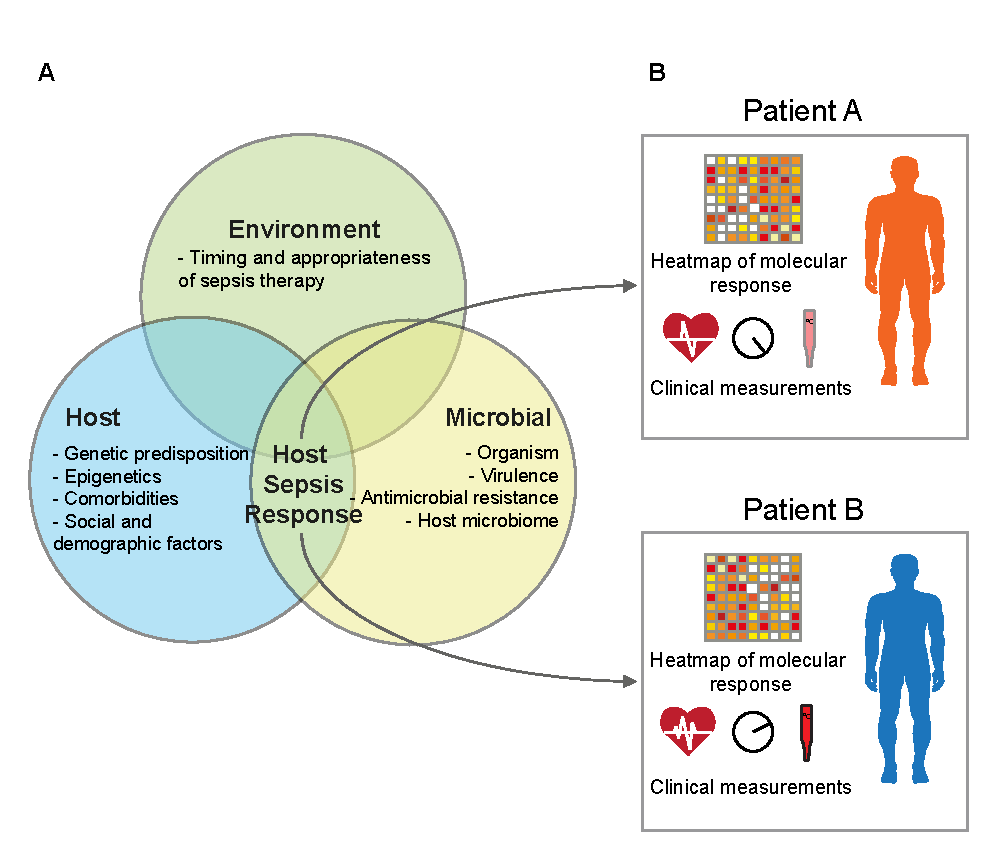
\includegraphics[scale=0.8]{./Introduction/Images/heterogeneity.pdf}
\caption[Heterogeneity in sepsis]{\textbf{Heterogeneity in sepsis.} Heterogeneity in the host response to sepsis can be resolved into clinically relevant endotypes. \textbf{A.} An interaction between host, environmental, and microbial factors leads to heterogeneity in the individual host response. \textbf{B.} This heterogeneity may be observed in the molecular and/or physiological response to sepsis, and may be resolved into patient subgroups or endotypes with clinically relevant and distinct disease phenotypes.}
\label{fig:heterogeneity}
\end{figure}

\subsection{Failure of clinical trials}
There has been overwhelming failure of over 100 Phase II and Phase III randomised clinical trials of therapies targeting the dysregulated inflammatory response in sepsis \parencite{Marshall2014}. These include drugs which:
\begin{enumerate}
\item Non-selectively suppress inflammation (e.g. ibuprofen \parencite{Bernard1997})
\item Neutralize microbial products (e.g. human anti-endotoxin monoclonal antibody \parencite{McCloskey1994})
\item Neutralize host inflammatory mediators (e.g. tumour necrosis factor receptor antagonist \parencite{Cohen1996})
\item Non-selectively target inflammatory mediators (e.g. intravenous immunoglobulins \parencite{Werdan2007})
\item Stimulate immune function (e.g. granulocyte colony-stimulating factor \parencite{Marti-Carvajal2012})
\item Have anticoagulant function (e.g. activated protein C \parencite{Root2003})
\end{enumerate}

Given the substantial heterogeneity seen in sepsis at both molecular and physiological levels, it is unsurprising that these trials have failed. All have used simple physiological parameters to identify the at-risk population and studied a reduction in mortality rate as a primary outcome. 

\subsection{Precision medicine approaches}
"Precision medicine" has been defined as \textit{"treatments targeted to the needs of individual patients on the basis of genetic, biomarker, phenotypic or psychosocial charaacteristics that distinguish a given patient from other patients with similar clinical presentations"} \parencite{Jameson2015}. 

In the context of sepsis, several examples indicate how a precision medicine approach may hold potential for benefit in clinical trials of sepsis therapy. In the example of drotrecogin alfa (recombinant human activated protein C), underlying host genetics may influence treatment outcome. A genome-wide association study (GWAS) of treatment response in sepsis patients receiving drotrecogin alfa identified several single nucleotide polymorphism (SNP) combinations in biologically relevant genes which were associated with a positive treatment outcome \parencite{Man2013}. In the top combination of three SNPs (observed in 26\% of the cohort), an large absolute risk reduction in 28-day mortality of 41.7\% was observed (compared with 6.1\% in the whole cohort). This result needs to be treated cautiously given the absence of a replication cohort. Nevertheless. the underlying principle is an important one; subgroups of individuals with certain genotypes might benefit from therapies that have been evaluated as non-efficacious in a heterogeneous cohort. 

A further example comes in the form of a post-hoc analysis of the Vasopressin vs Norepinephrine as Initial Therapy in Septic Shock (VANISH) trial \parencite{Antcliffe2019}. In this study, patients were randomised to receive norepinephrine or vasopressin followed by hydrocortisone or placebo. Patients were also categorized into two groups based on their peripheral blood leukocyte gene expression pattern, SRS1 (sepsis response signature 1) and SRS2. The authors observed an interaction between assignment to hydrocortisone or placebo, and SRS endotype (p=0.02) whereby hydrocortisone administration was associated with increased mortality in those with an SRS2 phenotype (odds ratio = 7.9; 95\% CI 1.6-39.9). This result is biologically plausible as individuals with the SRS2 phenotype were relatively immunocompetent compared to the SRS1 phenotype; abolishing this immunocompetent phenotype through the administration of the corticosteroid is likely to have been harmful. Again, this result illustrates how a precision medicine approach may be beneficial in trials of sepsis therapy by using transcriptomic signatures to select individuals who might benefit from a particular treatment.

\section{Omics-based approaches and the importance of the pathogen}

Omics-based methods have applied high-throughput techniques to enable understanding of the molecular mechanisms of sepsis from gene level to biological phenotype. Genomics, transcriptomics, epigenomics, proteomics, metabolomics, and metagenomics have all contributed to our understanding of sepsis pathophysiology and disease heterogeneity. 

In this section, I will illustrate how omics-based approaches as applied to sepsis will remain limited while studies using such approaches focus on the host to the exclusion of the pathogen. Examples from sepsis and other infectious diseases will be used to illustrate where efforts to account for the degree of heterogeneity involving the pathogen have led to valuable insights into host biology. 

\subsection{Genomics}
Three decades ago, a seminal epidemiological study \parencite{Sorensen1988} documented the surprising observation that premature mortality from severe infection is strongly heritable. Since then, a number of genomic approaches have been applied to studying the association between host genetics and sepsis susceptibility or disease outcome. Many of the results have been conflicting or underwhelming; a systematic review \parencite{Clark2006} of 76 candidate gene studies in sepsis assessed the majority of studies to be of low to moderate quality. Using Bayesian statistics, the authors calculated that 30 of the 32 SNPs associated with sepsis had at least a 50\% probability of being a false-positive finding if the prior probability of a true association was set at a liberal cutoff of 0.01.

Currently, there are only two reported GWAS of sepsis in the literature \parencite{Rautanen2015} \parencite{Scherag2016}; each of the studies identified different associations with 28-day survival. In the first study \parencite{Rautanen2015}, the reported association involved a SNP (rs4957796) located in an intron of the Fps/Fes related tyrosine kinase \textit{(FER)} gene on chromosome 5. Interestingly, this association reached significance only when cause of sepsis and microbiology was accounted for. Statistical significance was reached only when patients with sepsis from pneumonia were analysed independently from those with intra-abdominal infection (p combined=5.6x10$^{-8}$), with effect size increasing when bacterial cases of pneumonia were analysed separately (odds ratio reduced from 0.56 to 0.40, indicating increased effect size). \textit{FER} is implicated in sepsis-relevant pathways involving neutrophil chemotaxis and endothelial permeability; electroporation-mediated gene therapy of a plasmid containing the protective SNP imrpoves survival in murine models of traumatic lung contusion and pneumonia \parencite{Dolgachev2016}. However, two independent studies (a second genome-wide association study \parencite{Scherag2016} and a targeted validation study \parencite{Schoneweck2015}) have failed to replicate this association involving the \textit{FER} gene. 

The second GWAS \parencite{Scherag2016} analysed a wide range of infection types (lung, abdominal, urogenital, bone, soft tissue, and wound infections) and identified a different association (rs117983287) localising to the vacuolar protein sorting 13 homolog A \textit{(VPS13A)} gene on chromosome 9 (p=8.16x10$^{-8}$). Failure of replication between these genome-wide association studies, despite similar methods and outcome of interest, is potentially attributable to the different causes of sepsis investigated in each study. 

\subsection{Transcriptomics}
Transcriptomic studies in sepsis have aimed to define disease subphenotypes with distinct host response features. However, challenges in dissecting the various sources of disease heterogeneity have limited efforts to apply these studies to sepsis biomarker development. 

Studies comparing host transcriptomic signatures between different microbiological classes have yielded varying results. One study comparing neutrophil gene expression in ICU patients with Gram-positive and Gram-negative sepsis failed to identify significant differences \parencite{Tang2008}. This result is unsurprising given the small patient numbers (18 Gram-positive patients, 25 Gram-negative patients) and the diverse range of sepsis causes studied. For example, the Gram-negative group included many infection types (respiratory, intra-abdominal, urinary, and central nervous system) from ten different bacterial species. A unique transcriptome profile may have been observed if the authors had refined their analysis to a particular infection (e.g. respiratory) or pathogen type in a larger cohort of patients. 

A similar approach applied genome-wide gene expression profiling to peripheral whole blood in sepsis caused by acute respiratory illness. Three gene sets were defined that classified patients into bacterial, viral, co-infected, and non-infected causes with a classification accuracy superior to that of procalcitonin (87\% vs 78\%; p$<$0.03) \parencite{Tsalik2016}. 

Cheng and colleagues \parencite{Cheng2016} studied critically ill patients with sepsis who had proven \textit{Escherichia coli} bacteraemia and candida fungaemia. Analysis of peripheral blood gene expression microarray data showed that the majority of genes (5977) with significant differential expression from healthy volunteers (adjusted p$<$0.05) were common to both pathologies. Genes encoding proteins within pathways relevant to glycolysis and oxidative metabolism were upregulated in both groups. However, a unique transcriptional response specific to each pathogen was also seen (\textit{E. coli} bacteraemia, 1718 genes; candida fungaemia 830 genes). 

Multi-cohort analysis of publicly available transcriptomic data from patients with acute infection provides further evidence for distinct gene expression patterns depending on the pathogen \parencite{Sweeney2016}. Analysis of datasets from eight cohorts of patients enabled derivation of a seven-gene set, which discriminated bacterial from viral infection in 30 independent cohorts. In combination with a separate 11-gene set that discriminates infection from no infection \parencite{Sweeney2015}, the authors derived an antibiotics decision model that had 94\% sensitivity and 59.8\% specificity for bacterial infection. 

All these studies highlight the importance of accounting for underlying microbiological heterogeneity in studies of host gene expression in sepsis, such that any differences between study groups can be clearly distinguished from the signature attributable to the pathogen. 

\subsection{Regulation of gene expression}
Regulation of gene expression is dynamic, involving highly coordinated processes from transcription to post-translational stages. An extensive review of published GWAS identified that the majority of trait-associated and disease-associated SNPs were located in non-protein coding regions of the genome, with 88\% situated in intergenic or intronic regions \parencite{Hindorff2009}. These genetic variants are believed to contribute to the heritability of inter-individual variation in gene expression. In fact, SNPs associated with complex traits are more likely to be expression quantitative loci (eQTL) than frequency-matched SNPs \parencite{Nicolae2010}. Given that eQTL show strong heritability \parencite{Wright2014}, these regulatory genetic variants could reflect the major selective pressure that pathogens have exerted on human genetics. 

Quantitative trait loci mapping approaches define the association of a SNP with an intermediate phenotype (e.g. levels of a transcript (eQTL), protein, or metabolite). These approaches have convincingly shown the importance of cellular context and environment on the activity of a regulatory variant. For example, in-vitro studies of human monocytes exposed to biological stimuli relevant to bacterial (lipopolysaccharide) and mycobacterial or viral (interferon-$\gamma$) infections have shown that exposure to these stimuli is necessary to show the association of SNPs with the expression of innate immune system-related genes \parencite{Fairfax2014}. In some examples, the direction of effect on gene expression (i.e. an increase or decrease in gene expression) can even differ between different conditions. A similar approach applied to human primary dendritic cells exposed to mycobacterium tuberculosis identified 198 loci associated with gene expression that were not observed in unstimulated cells, reflecting the effect of the host-pathogen interaction \parencite{Barreiro2012}. 

These observations are highly relevant to studies of sepsis patients, where we must consider the biological context set by a particular infecting pathogen and its influence on underlying host genomic modulation of gene expression. In a study of GAinS ICU patients with sepsis from CAP \parencite{Davenport2016} there was evidence of eQTL in genes associated with viral respiratory infection. This was observed even though only 9\% of patients within this cohort had CAP of confirmed viral cause; this analysis would have been enhanced by more detailed microbiological phenotyping of the cohort. 

The relevance of non-coding RNAs in the regulation of gene expression has become increasingly recognised. MicroRNAs (miRNAs) have been of particular interest as potential biomarkers in sepsis. However, conflicting results pose a challenge for the interpretation and application of these studies. For example, significantly reduced miR-223 levels were observed in one cohort of patients with sepsis, compared with patients with systemic inflammatory reponse syndrome and healthy individuals \parencite{Wang2010}, while elevated miR-223 levels were observed in another cohort of patients with sepsis compared with healthy individuals \parencite{Wang2012}. In a third study \parencite{Benz2015}, no differences in miR-223 levels were found between individuals with and without sepsis. The authors of the third study attribute these conflicting results to important difference in methods of normalisation. However, differences in cause of infection deserve consideration. The first of these three studies included only ICU surgical patients with intra-abdominal and trauma-related infection, whereas the other two recruited patients with respiratory infection and a broader range of infective pathologies. Even within the context of different strains of the same virus, significant differences in miR-223 expression can be observed. In mice infected with a reconstructed pandemic 1918 H1N1 influenza A virus, distinct patterns of lung tissue miRNA expression were observed compared with those infected with a seasonal H1N1 influenza A virus (strain A/Texas/36/91) \parencite{Li2010}. Specifically, levels of miR-223 were nearly three-times higher with the pandemic strain than with the seasonal strain.

\subsection{Proteomics and metabolomics}
Advances in mass-spectrometry-based methods enables large-scale analysis of the protein and metabolite composition of biological samples in sepsis research. There is the potential for unique functional insights beyond those afforded by genomics and transcriptomics since there is no direct association between mRNA expression and protein or metabolite levels.

Langley and colleagues \parencite{Langley2013} studied patients presenting to the emergency department with suspected community-acquired sepsis. Unique plasma proteomic and metabolomic profiles were seen in the three groups of patients: sepsis survivors, sepsis non-survivors, and individuals with a non-infective systemic inflammatory response syndrome. Non-survivors had profiles indicative of impaired mitochondrial fatty acid $\beta$ oxdiation. The authors of this study developed a prognostic logistic regression model based on seven parameters (four carnitine esters, lactate, age, and haematocrit). This model was validated in two separate cohorts and successfully classified sepsis survivors and non-survivors with an accuracy of 85\%, superior to that of lactate, Sequential Organ Failure Assessment, or Acute Physiology and Chronic Health Evaluation II scores. Interestingly, no substantial differences were seen between the plasma metabolome and proteome of patients with sepsis due to \textit{Streptococcus pneumoniae}, \textit{Staphylococcus aureus} and \textit{Escherichia coli}. The authors postulated that this might have been because of heterogeneity with respect to infection site, and the possibility that subtle differences were overwhelmed by a generalised septic response. Indeed, in a different cohort of patients with Gram-positive and Gram-negative sepsis, ELISA-based quantification of a more limited panel of 11 plasma cytokines showed higher interleukin-1$\beta$, interleukin-6 and interleukin-18 concentrations in the Gram-positive group compared with the Gram-negative group \parencite{Feezor2003}. In another study \parencite{Huang2014}, recruiting a more homegeneous cohort of Gambian children with pneumonia, a mass-spectrometry-based proteomic analysis identified 42 proteins that differentiated severe from non-severe pneumonia and non-severe pneumonia from controls \parencite{Huang2014}. One of these proteins was neutrophil gelatinase-associated lipocalin (lipocalin-2), which discriminates pneumonia of probable bacterial cause from viral cause. Children with plasma concentrations of lipocalin-2 more than 163 ng/ml were nine times more likely to have a positive blood culture with a clinically significant isolate. Proteomic and metabolomic studies of sepsis represent a rich, untapped source of potential disease biomarkers for the clinical setting. 

\subsection{Epigenetics}
From the perspective of evolutionary biology, the co-existence of pathogen and host is a major selective pressure on the genetic diversity of both organisms \parencite{Sironi2015}. While random point mutations in DNA (SNPs) are a key source of diversity, the role of epigenetic changes in contributing to more rapid changes to organism phenotype is being increasingly recognised \parencite{Rando2007}. Both viruses \parencite{Paschos2010} and bacteria \parencite{Hamon2008} have the potential to induce epigenetic changes in humans, modulating the biological interaction between pathogen and host with significant consequences to disease course.

For example, the H3N2 influenza A virus carries a histone-like sequence in its non-structural protein 1 (NS1) tail. This allows it to interact with the host epigenome;   binding of the NS1 protein to the human polymerase associated factor 1 transcription elongation complex allows the virus to target sites of actively transcribed antiviral genes, suppressing the antiviral response \parencite{Marazzi2012}. Interestingly, the H1N1 influenza A virus does not possess this histone-like NS1 tail, which might explain the different disease phenotypes seen between various strains.

There are few epigenetics studies of sepsis. However, there is substantial corroborative evidence to support epigenetics as a promising approach to advance our understanding of the disease. In an animal model of acute lung injury and sepsis, anaesthetised mice were exposed to a dual pulmonary insult of aspiration of a \textit{Staphylococcus aureus} culture and mechanical ventilation \parencite{Bomsztyk2015}. After only 6 hours, there was decreased expression of the angiogenic genes \textit{ANGPT1, TEK,} and \textit{KDR} in the lung, kidney, and liver. Chromatin immunoprecipitation assays showed a decrease in relative RNA polymerase II abundance and histone deacetylation at these genes, providing evidence for the role of epigenetic changes in contributing to sepsis-induced endothelial dysfunction.

In the previously mentioned study of gene expression in adult ICU patients with sepsis due to CAP \parencite{Davenport2016}, the locations of the observed sepsis eQTL showed substantial overlap with epigenetic marks observed in monocytes stimulated with bacterial lipopolysaccharide. This overlap included deoxyribonuclease (DNase) I hypersensitive sites (i.e regions of chromatin where DNase I activity results in the DNA being accessible to transcription factor binding) and histone marks associated with enhancer and promoter regions (i.e. specific covalent modifications such as H3K27ac, H3K4me1, H3K4me3).

In summary, results from studies in animal models and in humans with sepsis suggest a strong role for epigenetic changes in sepsis pathophysiology. However, to translate these changes to patient benefit (e.g. identification of novel therapeutic targets), these epigenetic mechanisms will need to be dissected further. Studies that take account of specific infection types will be an important way to achieve this aim.

\subsection{Metagenomics}
Unique host and pathogen factors interact to result in the heterogeneous sepsis immune response. However, this host-pathogen interaction does not occur in isolation but within a rich microbial context. The term pathobiome illustrates this concept - that a microorganism's pathogenicity depends not just on its specific virulence factors, but also on host factors, environmental factors, and the microbial community of which it is a part \parencite{Vayssier-Taussat2014}. 

Advances in metagenomics has been facilitated by the increasing affordability of high-throughput sequencing. Of relevance to sepsis is the mechanisms by which one microorganism (or a community of microorganisms) can influence the interaction of another microorganism with the host. This synergism between multiple pathogens is well-recognised in influenza virus infection, where adherence of \textit{Streptococcus pneumoniae} to the respiratory epithelium is facilitated by viral neuraminidase \parencite{Peltola2005}. Metagenomics now enables the consideration of synergism beyond a handful of organisms, by revealing new mechanisms through which the whole microbiome influences host susceptibility to infection.

Mucosal surfaces represent a critical interface for the microbiome-host interaction; microorganisms previously considered to be pure commensals act both directly and indirectly at sites such as the intestinal and respiratory epithelium to protect the host from potentially pathogenic organisms. Directly, the intact microbiome provides a barrier effect by limiting the supply of essential resources at these sites. Indirectly, the microbiome interacts with immune cells at mucosal surfaces, leading to the modulation of key innate and adaptive immune pathways \parencite{Thaiss2016}. In murine models, the bacterial component of the gut microbiome plays an essential part in enabling persistent norovirus infection by limiting the efficacy of interferon-$\gamma$ mediated innate immunity \parencite{Baldridge2015}. Adaptive immunity is also mediated by the microbiome, with the response to influenza virus shown to depend on a healthy lung bacterial microbiome. Mice receiving a 4-week course of oral antibiotics developed marked dysbiosis of the lung microbiome, leading to defective CD4 T-cell, CD8 T-cell, and B-cell mediated immunity to subsequent intranasal influenza virus challenge \parencite{Ichinohe2011}. This suggests that antibiotics might be not just unnecessary, but actually harmful in cases of viral respiratory infection with potentially serious implications in patients with chronic lung conditions (e.g. chronic obstructive pulmonary disease or cystic fibrosis), who frequently receive antibiotics as prophylaxis or for treatment of exacerbations. 

Large-scale endeavours such as the National Institutes of Health Human Microbiome Project \parencite{Peterson2009} have revealed the extent to which the microbiome differs between healthy individuals. This diversity is often lost in critical illnesses such as sepsis, in which both disrupted host pathophysiology and clinical interventions to manage the underlying condition result in striking changes to the microbiome \parencite{Dickson2016}. There is convincing evidence to suggest that host genetic variants interact with the microbiome to result in the development of immune-related disease; for example, K/BxN transgenic mice do not develop inflammatory arthritis in a germ-free environment since segmented filamentous bacteria in the gut are essential to T-helper-17 cell activation and subsequent joint inflammation \parencite{Wu2010}. This could have implications in sepsis, in which the relevance of host genetics to disease might be better understood in the context of inter-individual differences in the microbiome.

There is potential for metagenomic analysis of the microbiome to yield prognostic information in sepsis: in conditions as diverse as bronchiectasis \parencite{Rogers2014} and metabolic syndrome \parencite{LeChatelier2013}, the microbiome has been shown to correlate with disease phenotype and outcome. Metagenome-wide association studies \parencite{Zhang2015} that identify associations between microbial genes and disease traits have found that restoration of dysbiosis in the dental microbiome is associated with good response to disease-modifying anti-rheumatic drugs in rheumatoid arthritis. It is not inconceivable that microbiome-based tests could similarly be identified as biomarkers for early diagnosis, patient stratification, and evaluation of treatment response in sepsis. Additionally, the microbiome represents an attractive therapeutic target in sepsis, with murine models showing a reduction in criculating aged neutrophils following antibiotic depletion of the gut-microbiota, with corresponding improvements in survival from endotoxin-induced septic shock \parencite{Zhang2015a}. As an important source of heterogeneity in sepsis, characterisation of the microbiome and integration of this second genome \parencite{Grice2012} into other omics-based approaches should be a key priority in further sepsis research.

\section{New opportunities in clinical microbiology}
A USA-based epidemiological study \parencite{Gupta2016} of nearly 7 million sepsis patients hospitalised between 2001 and 2010 estimated the incidence of culture-negative sepsis at 47\%, with culture negativity identified as an independent predictor of mortality. Making a microbiological diagnosis is a key clinical priority, enabling effective antimicrobial therapy within the framework of responsible stewardship. Emerging new technologies bring the potential of more rapid and detailed resolution of microbiology in sepsis, and can be classified into one of three main approaches: PCR-based techniques, mass-spectrometry-based methods, and nucleic acid sequencing (next-generation or high-throughput sequencing) methods.

\subsection{Multiplex PCR}
Multiplex PCR platforms enable the simultaneous detection of multiple pathogens with high sensitivity and specificity. Antimicrobial susceptibility data can be provided and there is potential for automation. Point-of-care platforms are being increasingly commonplace in the clinical setting with the advantage of rapid turnaround times and user-friendly sample processing. 

The BioFire FilmArray (bioMerieux, Marcy l'Etoile, France) respiratory \parencite{Xu2013} and meningitis/encephalitis \parencite{Lee2019} panels are two examples of disease specific multiplex PCR platforms. The respiratory panel \parencite{Xu2013} tests for 15 viral pathogens in respiratory specimens and was implemented in a regional paediatric hospital in the USA with a median turnaround time of 1.4 hours. Over 2,500 specimens were tested by FilmArray and a direct fluorescence assay in parallel. The FilmArray panel detected rhinovirus in 20\% of samples and coronavirus in 6\% of samples, both organisms were not part of the direct fluorescence assay panel. Whilst the respiratory panel only tests for viruses, the meningitis/encephalitis panel tests for 14 pathogens, including 6 bacteria, 7 viruses, and 1 fungal species from cerebrospinal fluid \parencite{Lee2019}. Forty-two individuals presenting to the emergency department with relevant symptoms were tested using the FilmArray platform; six positive samples were detected with an 88\% agreement rate with conventional microbiology testing.

There are two main disadvantages with these platforms. Firstly, detection is limited to pathogens in the pre-specified probe panel, which are limited in their scope. Therefore, the platforms are limited in geographical locations where there is a high prevalence of infection caused by microorganisms not included in the panel. Secondly, false-negative results may arise where variation among pathogen genomes leads to failure to detect the organism. For example, a variant strain of \textit{Chlamydia trachomatis} in Sweden led to false negative testing by PCR \parencite{Ripa2006} because the variant strain had a deletion of 377bp in the cryptic plasmid, the region targeted by PCR testing.

\subsection{Mass spectrometry}
There are generally two methods of mass spectrometry applied to microbiological testing: matrix-assisted laser desorption ionisation-time of flight mass spectrometry (MALDI-TOF) and electrospray ionisation-mass spectrometry (ESI-MS) \parencite{Buchan2014}. The difference in the two techniques lies in the generation of the ions. In MALDI-TOF, the analyte is allowed to dry before being overlaid by a weak acid matrix material. It is then exposed to a laser which ionises and desorbs it from the sample plate. The created ions are then accelerated through a vacuum by the application of an electrostatic field. In contrast, analytes need to be in the liquid phase for ESI-MS. The solute is passed through a heated capillary and exposed to a high voltage to generate an aerosol of ions. 

Huang and colleagues compared MALDI-TOF and antimicrobial stewardship team (AST) intervention with routine clinical care in individuals with bloodstream infection \parencite{Huang2013}. Routine clinical care included analysis of blood culture results using the VITEK-2 system (biochemical testing for antimicrobial susceptibility information) without AST intervention. In the study group, the AST intervention consisted of provision of evidence-based antimicrobial recommendations after receiving a positive result. The intervention group showed significantly decreased time to organism identification, decreased time to effective antimicrobial therapy, decreased 30-day mortality and decreased ICU length of stay, compared with the pre-intervention control group.

ESI-MS has also been studied in individuals with bloodstream infection \parencite{Vincent2015}. In 616 individuals with bloodstream infection, ESI-MS identified a pathogen in 37\% of individuals compared with a 11\% diagnostic rate for blood cultures. An expert panel was enlisted to provide independent clinical analysis and concluded that ESI-MS could potentially have altered treatment in up to 57\% of patients.

\subsection{Nucleic acid sequencing}
See next section (Section \ref{sec:clinmetagenomics}) for a description of short-read nucleic acid sequencing.

\subsection{Nanopore sequencing}
Nanopore sequencing is an emerging NGS technology that performs long-read sequencing with real-time sequence analysis \parencite{Jain2016}. Commercially available platforms include the MinION (1 flow cell), GridION (5 flow cell capacity), and PromethION (48 flow cell capacity). The MinION has been successfully applied to outbreak surveillance, e.g. in epidemiological outbreak surveillance of Ebola virus in west Africa \parencite{Quick2016} and Salmonella in a UK-based inpatient setting \parencite{Quick2015}.

Examples of application to diagnostics in clinical syndromes remains limited due to inherent challenges; MinION sequencing has been applied to urinary tract infections \parencite{Schmidt2017}, prosthetic joint infections \parencite{Sanderson2018}, and lower respiratory infections \parencite{Charalampous2019}. Schmidt and colleagues \parencite{Schmidt2017} analysed 10 heavily infected urine specimens ($>$10$^7$ cfu/ml) and 5 specimens of healthy urine spiked with multi-drug resistant \textit{Escherichia coli}. With a turnaround time of 4 hours, there was 100\% agreement between MinION sequencing result, Illlumina sequencing, and clinical microbiology. In addition, 51/55 resistance genes detected by Illumina sequencing were found by minION sequencing. However, the authors noted a number of limitations with their study, including the fact that only heavily infected urine was analysed, the cost of sequencing (only one sample was sequenced per flow cell) and the poor identification of allelic variants and resistance-conferring mutations due to poor base-calling accuracy. Compared to Illumina sequencing, the potential for scalability in terms of number of samples and data volumes remains relatively limited in Nanopore sequencing.  

\section{Clinical metagenomics} \label{sec:clinmetagenomics}
Clinical metagenomic next-generation sequencing has been described as the characterisation of \textit{``all DNA and/or RNA present in a sample, enabling analysis of the entire microbiome as well as the human host genome or transcriptome in patient samples"} \parencite{Chiu2019}. 

\subsection{Applications}
\textbf{Infectious disease diagnostics.} NGS approaches can be untargeted or targeted in their approach. Untargeted approaches involve the sequencing of the entire DNA and/or RNA component of a sample. Typically, $>$99\% of the reads obtained are human in origin, so sensitivity for a pathogen can be a critical issue. However, advantages include the unbiased nature of the approach, enabling comprehensive analysis of all pathogens in a single assay. 

Targeted approaches include the following three approaches: (i) targeted PCR amplification of a conserved region (e.g. 16S ribosomal RNA (rRNA) gene amplification for bacteria \parencite{Watanabe2018}, and 18S rRNA and internal transcribed spacer gene amplification for fungi \parencite{Wagner2018}), (ii) targeted PCR amplification of a whole genome using tiled primers \parencite{Quick2017}, and (iii) hybrid-capture based techniques whereby metagenomic libraries are subjected to hybridisation using capture "bait" probes \parencite{Bonsall2015}. Targeted approaches are able to increase the proportion of pathogen reads in the sequence data, thereby increasing sensitivity with potential reductions in cost of sequencing because less total sequencing reads are required to achieve a given depth of pathogen coverage.

\textbf{Clinical microbiome analysis.} There is increasing awareness of the role of the microbiome in the pathogenesis of both acute and chronic illnesses. One group charcterised the microbiome of blood in sepsis (n=62) patients and healthy volunteers (n=23) \parencite{Gosiewski2017}. The authors observed striking differences between the taxonomic composition of the two groups; the microbiome of healthy volunteers was composed of mainly anaerobic bacteria whereas the microbiome of septic patients was composed of mainly aerobic and microaerophilic microorganisms. There was decreased representation of the Actinobacteria phyla in sepsis patients and decreased representation of the Proteobacteria phyla in healthy volunteers. 
 
\textbf{Human transcriptomic analysis.} Although clinical metagenomics focuses on the microbial reads recovered from a sample, analysis of human gene expression is also possible if RNA libraries have been constructed from the clinical samples. This incidental RNA-seq data has the potential to inform analysis of pathogen reads. For example, infective and non-infective pathologies can be differentiated by combined host and pathogen read data analysis. Clinical metagenomic NGS of tracheal aspirate samples enabled differentiation of individuals with acute respiratory failure from lower respiratory tract infections versus those with non-infectious causes based on pathogen, microbiome diversity, and host gene expression metrics \parencite{Langelier2018a}. Also, dual transcriptome analysis enables improved understand of host-pathogen interactions. Analysis of Gambian children infected with \textit{Plasmodium falciparum} revealed distinct human and parasite gene expression profiles associated with severe malaria phenotypes \parencite{Lee2018}. Up to 99\% of human differential gene expression was driven by differences in parasite load and coexpression analyses revealed interactions between host and parasite, with marked co-regulation of translation genes in severe malaria. Furthermore, RNA-seq can be especially useful in cases of infection where the causative pathogen is only transiently present in the host, e.g. Lyme disease \parencite{Marques2015} or Zika virus infection \parencite{Landry2017}, since distinct pathogen-specific human transcriptomic signatures may be identified.

\textbf{Applications in oncology.} Sequencing of tumour samples can be used to identify viruses associated with cancer (e.g. herpesviruses, papillomaviruses, and polyomaviruses) and also to identify virus-host interactions. For example, metagenomic NGS enabled the identification of a previously unknown polyomavirus, Merkel cell polyomavirus, in skin tissue analysis of Merkel cell carcinoma (a rare but aggressive dermatological cancer) \parencite{Feng2008}. In addition, targeted metagenomic sequencing enabled eight whole genomes of Epstein-Barr virus to be sequenced from primary nasopharyngeal carcinoma biopsy specimens \parencite{Kwok2014}. Clinical metagenomics may also inform the treatment of cancers associated with viral infection. For example, Kanwal and colleagues \parencite{Kanwal2017} showed that in hepatitis C virus patients treated with direct-acting antiviral agents, those with sustained virological response showed a reduction in the risk of hepatocellular carcinoma.

\subsection{Hybrid-capture based techniques}
Of the three approaches to targeted metagenomics described above, the hybrid-capture based technique is the most versatile as it does not depend on the specificity of highly conserved primers for PCR amplification. The capture procedure is typically applied after nucleic acid extraction and library preparation. Here, RNA baits are preferable to DNA baits as RNA:DNA duplexes hybridise with greater efficiency and stability than DNA:DNA hybrids \parencite{Lesnik1995}. The hybridisation can be carried out on a solid support (i.e. array-based) \parencite{Schuenemann2018}, or more commonly, in-solution \parencite{Briese2015}. For the in-solution technique , biotinylated baits bind the target of interest \parencite{Gnirke2009}. Then, Streptavidin coated magnetic beads are added to the solution, which bind to the biotinylated baits. Subsequent washing steps lead to non-specific unbound molecules being washed away before the sample is sent for NGS. 

Hybrid-capture based techniques have been applied to clinical metagenomic NGS of bacteria \parencite{Allicock2018}, viruses \parencite{Depledge2011} \parencite{Briese2015} \parencite{Wylie2015}, fungi \parencite{Amorim-Vaz2015}, and parasites \parencite{Bright2012}. 

For bacterial sequencing, the BacCapSeq platform includes a probe set comprised of 4.2 million oligonucleotide probes which enable detection and characterisation of bacteria, virulence determinants and antimicrobial resistance genes \parencite{Allicock2018}. The capture resulted in up to a 1000-fold increase in sensitivity with blood samples.

For viral sequencing, the first example of hybrid-capture based NGS involved a study which targeted three full length herpesvirus genomes (Varicella-Zoster Virus, Epstein-Barr virus and Kaposi's sarcoma-associated Herpesvirus) \parencite{Depledge2011}. A range of clinical sample types were tested across 13 samples and full length herpesvirus genomes reconstructed at high read depth. Other examples of hybrid-capture based NGS applied to viruses include ViroCap \parencite{Wylie2015} and VirCapSeq-VERT \parencite{Briese2015}. Virocap includes a panel of probes designed to enrich for nucleic acid from 34 families of DNA and RNA viruses (190 viral genera and 337 species) that infect vertebrate hosts, excluding human endogenous retroviruses \parencite{Wylie2015}. The authors showed that the probes only required a minimum of 58\% probe-target homology for enrichment and sequencing. VirCapSeq-VERT includes 2 million probes covering 207 viral taxa that infect vertebrates \parencite{Briese2015}. The authors demonstrated that the capture resulted in a 100- to 10,000-fold increase in viral reads from blood and tissue homogenates compared to conventional Illumina sequencing using established virus enrichment procedures (filtration, nuclease treatments, and RiboZero rRNA subtraction). Novel viruses were also detected where their genomes were approximately 60\% similar to probes included in the capture library.

For fungal sequencing, Amorim-Vaz and colleagues \parencite{Amorim-Vaz2015} designed a set of 55,342 probes covering 6,094 \textit{Candida albicans} open reading frames. Results showed approximately 1000-fold enrichment of \textit{C. albicans} reads in biological samples and a detection of more than 86\% of its genes. 

For parasite sequencing, \textit{Plasmodium vivax} enrichment enabled an increase in sequencing yield from 0.5\% to a median of 55\%, with 5X coverage across 93\% of the \textit{P. vivax} genome \parencite{Bright2012}.

\subsection{Application to sepsis}
Apart from the work described in this thesis \parencite{Goh2019}, there are several recent examples in the literature of clinical metagenomics as applied to adult sepsis patients. None of these examples include the simultaneous sequencing and analysis of bacterial, DNA viral, and RNA viral reads. 

Blauwkamp and colleagues \parencite{Blauwkamp2019} performed microbial cell-free DNA sequencing from the plasma of 348 adult patients presenting to the Emergency Department who met sepsis alert criteria. Next-generation sequencing (NGS) yielded a positive diagnosis in 49\% of individuals, compared to an 18\% diagnostic yield from blood cultures and 38\% diagnostic yield from all conventional microbiological testing combined. The method only enabled identification of bacteria, DNA viruses, fungi, and eukaryotic parasites. NGS was particularly helpful in identifying a cause of sepsis in patients who had received preceding antibiotics when compared to conventional microbiological testing. The authors also describe their experience of NGS processing of the first 2000 plasma samples submitted to their Clinical Laboratory Improvement Amendments certified and College of American Pathologists accredited laboratory. They achieved a 98\% rate of sample reporting within one day after sample receipt.

In a smaller study, Grumaz and colleagues \parencite{Grumaz2019} also applied cell-free DNA sequencing to plasma from septic shock patients (n=48). NGS yielded a diagnosis in 72\% of individuals compared to a 33\% diagnostic rate from blood cultures. A clinical expert panel reviewed the NGS results; 96\% of NGS results were deemed plausible and were judged to have led to a change to more adequate therapy in 53\% of cases.

In six Vietnamese hospitals, NGS was applied to 492 clinical samples from 386 patients with community acquired sepsis \parencite{Anh2019}. A range of sample types were sequenced including serum, nasal/throat swabs, stool and cerebrospinal fluid. Only sequencing reads aligning to viral sequences were analysed. The authors confirmed each positive NGS result with PCR and considered only those validated by PCR as positive. 21 viral species known to be infectious in humans were identified in 13.4\% of patients.

Finally, a study of Chinese ICU patients with sepsis (n=78) described the preparation of DNA libraries from plasma and Ion Torrent sequencing \parencite{Long2016}. NGS yielded a 31\% diagnostic rate versus 13\% from blood cultures. 

\subsection{Challenges}
There are a number of challenges associated with clinical metagenomics, which will be described in this section.

\textbf{Sensitivity.} As discussed above, typically $>$99\% of metagenomic NGS reads generated originate from the host. This is because the majority of nucleic acid in clinical specimens is human in origin, and also because human genomes are far larger than that of bacteria and viruses. Strategies to increase sensitivity for microbial reads include targeted metagenomic approaches (described above) as well as other purification or enrichment procedures to increase pathogen yield. For bacterial pathogens, the most common first step is culture, which can favour contaminating, culturable or fast-growing organisms. For viral pathogens and some bacteria, yield-maximising methods include filtration to remove host cells \parencite{Allander2001}, sample treatment with nucleases to digest nucleic acid not protected within cells or virions \parencite{Allander2001} \parencite{Charalampous2019}, and high-speed gradient centrifugation to concentrate virus particles \parencite{Breitbart2005}. Each of these procedures reduces throughput and may bring about bias.

\textbf{Interpretation of positive results.} In the context of a metagenomic positive result, it can be challenging to differentiate infection from colonisation or contamination. In certain samples (e.g. respiratory specimens), the normal microbiota can be rich and complicate interpretation of results. Systematic PCR testing of nasopharyngeal or bronchoalveolar lavage specimens from patients in intensive care, admitted with pneumonia, identified respiratory viruses in over a third of patients, the relevance of which remains uncertain \parencite{Choi2012}. One potential solution is the use of spike-in based calibration to enable quantitative analysis through conversion of percentage reads to colony-forming units per milliliter \parencite{Stammler2016}. Another approach is to assess the host immune response by simultaneous analysis of the human transcriptome. Langelier and colleagues evaluated a composite metric of immunity genes in haematopoietic cellular transplant patients as a biomarker of active infection, using this to differentiate colonisation from active infection \parencite{Langelier2018}. 

The use of controls (healthy individuals as well as no-template controls) can also be a useful strategy, especially for differentiating causative pathogens from extraneous sources of DNA ubiquitous in commonly used reagents used in the extraction and library preparation procedures \parencite{Salter2014}. For example, Grumaz and colleagues \parencite{Grumaz2016} assigned a sepsis indicating quantifier score to each identified microbe in a sample, to indicate the probability of it being a true positive finding (on the basis of the number of reads mapping to the microbe's reference genome in the patient sample, relative to healthy individuals). A further approach is to evaluate the proportion of the genome covered by the reads mapping to an organism; where reads are localised to limited regions of the genome, this is more likely to represent contamination when compared to reads spanning larger regions of the genome.

\textbf{Turnaround times.} Time from sample receipt to data generation can vary, and has been reported to be anywhere from 6 hours to 7 days (average 48 hours) \parencite{Simner2018}. These long turnaround times arise because of laborious library preparation stages essential to making a clinical sample suitable for sequencing as well as time taken for the generation of sequence data. However, automated processes are becoming increasingly commonplace and new technologies, such as Oxford Nanopore Technologies, require less pre-processing and provide real-time data analysis \parencite{Quick2016}. 

\textbf{Data analysis.} A sizeable gap exists between the generation of NGS data and the analysis and processing of this data to generate clinically relevant information. Although bioinformatic pipelines have been implemented in clinical settings (e.g. the sequence-based ultrarapid pathogen identification SURPI pipeline \parencite{Wilson2019}), there is still lack of standardisation of data processing and analysis methods. In addition, bioinformatics packages and pipelines currently require a substantial degree of bioinformatics expertise that is not routinely available in clinical settings. 

The absence of well-curated databases also poses a challenge. Draft and partial genomes on NCBI (National Centre for Biotechnology Information) may lead to erroneous results. For example, false positive results may arise from mapping to low complexity regions in the reference sequence or to contaminants from database entries that contain reads to human DNA or sequencing adapters. Also, false negative results may arise due to incomplete or missing taxonomic representation in databases.

\section{Specific aims and objectives}
The aims of this thesis are to:

\begin{itemize}[leftmargin=*]

\item	\textbf{Develop a library preparation method for metagenomic sequencing of plasma samples 
(\hyperref[ch:Results1]{Ch. 3})} \\
Commercially available library preparation methods are available for either RNA or DNA, but not both within a single streamlined method. Sensitivity is likely to be a limiting factor in metagenomic sequencing from plasma; hybrid-capture based techniques provide an opportunity to improve sensitivity. I aim to:

		\begin{enumerate}
		\item Use probe-based enrichment to increase sensitivity for sequencing organisms relevant to sepsis due to CAP from plasma
		\item Optimise a library preparation method suitable for sequencing both DNA- and RNA-based organisms from plasma
		\item Evaluate performance of the library preparation method against a known positive control reference set
		\end{enumerate}
		
\item	\textbf{Improve definition of microbiological aetiology using targeted metagenomics, PCR-based pathogen analysis, and clinical data (\hyperref[ch:Results2]{Ch. 4})} \\
Various methods can be used to improve the microbiological diagnosis rate in GAinS CAP sepsis patients. I aim to improve microbiological classification of GAinS CAP sepsis patients through:

		\begin{enumerate}
			\item Application of targeted metagenomics to plasma samples
			\item Use of droplet digital PCR to assay \textit{Streptococcus pneumoniae} and Epstein-Barr virus from plasma samples
			\item Use of the Axiom Microbiome Array
		\end{enumerate}

\item	\textbf{Improve characterisation of disease heterogeneity in patients with no previous microbiological diagnosis through integrated application of metagenomic, transcriptomic and genomic techniques (\hyperref[ch:Results3]{Ch. 5})} \\
Integrated -omic approaches have the potential to enhance our understanding of the heterogeneous host response in sepsis. In this chapter, I aim to:
		\begin{enumerate}
			\item Characterise the extent and implications of EBV reactivation and integrate this with host transcriptomic data
			\item Investigate the association between \textit{Streptococcus pneumoniae} bacterial load and sepsis endotype (SRS status)
			\item Describe host transcriptomic signatures of viral infection, influenza infection, and \textit{Streptococcus pneumoniae} infection
			\item Investigate the association between host genotype (HLA type) and susceptibility to different classes of infection
		\end{enumerate}

		
\end{itemize}







										
\cite{Bonsall2015}
\chapter{Materials and Methods}
\label{ch:MandM}
\textit{This chapter describes the patient cohorts, laboratory methods, and bioinformatic methods used in this thesis}

\startcontents[chapters]{\vspace{-1.4cm}}
\singlespacing
\printcontents[chapters]{}{1}{\section*{ }\setcounter{tocdepth}{1}}
\doublespacing

\section{Genomic Advances in Sepsis}
The UK Genomic Advances in Sepsis (GAinS) study (http://ukccggains.com) is a multicentre prospective study initiated in 2005 by the UK Critical Care Genomics group with the original aim of characterising genetic variants that affect susceptibility to and outcomes from sepsis. A bioresource arising from this study includes biological samples and phenotypic information from over 2,000 individuals with sepsis from community acquired pneumonia (CAP) or faecal peritonitis (FP) admitted to intensive care units (ICUs). This thesis focuses only on the subset of individuals with sepsis from CAP. Recruitment was initially carried out in 34 ICUs and remains ongoing in 4 ICUs across the UK.

\subsection{GAinS patient recruitment and exclusion criteria}
Sepsis patients were recruited through the GAinS study from 34 participating ICUs between 2005 and 2019. Patients were recruited if they met the diagnostic criteria for severe sepsis in use at the time of study initiation (Sepsis-2, 1992 American College of Chest Physicians/Society of Critical Care Medicine consensus definition \parencite{Bone1992}). CAP was defined as febrile illness associated with cough, sputum production, breathlessness, leukocytosis and radiological features of pneumonia acquired prior to or within 48 hours of hospital admission \parencite{Lim2009}. Exclusion criteria included immunocompromise, admission for palliative care only, and pregnancy.

\section{Additional cohorts}
Two other cohorts were studied: (a) patients with hepatitis C virus infection, and (b) patients undergoing cardiac surgery.

\subsection{Hepatitis C virus infection patient recruitment and exclusion criteria}
The hepatitis C virus infection (HCV) cohort was recruited through the NIHR Oxford Biomedical Research Centre Prospective Cohort Study in Hepatitis C. 

\subsection{Cardiac surgery patient recruitment and exclusion criteria}
Patients undergoing elective cardiac surgery requiring cardiopulmonary bypass (coronary artery bypass grafting, valve replacement, or valve repair) were recruited to the Genomic Advances in Cardiac Surgery study by Dr Eduardo Svoren and Professor Charles Hinds (Bart's and the London NHS Trust). This study aimed to investigate the host inflammatory response induced by elective cardiac surgery involving cardiopulmonary bypass. They were included in this thesis as uninfected negative controls for sepsis. Patients were excluded if they were immunocompromised, undergoing an emergency operation, had malignancy, or were unable to provide informed consent. 


\section{Metagenomics}
\subsection{Nucleic acid extraction}

Total nucleic acid extraction was performed using the NucliSENS easyMag platform (Biomerieux). Typically, 500 $\mu$l of extracted plasma was eluted in 25 $\mu$l of buffer. Postextraction quality control was performed using the Agilent 2100 Bioanalyzer platform and/or the Qubit dsDNA High Sensitivity Assay (Thermo Fisher Scientific) in a subset of samples.

\subsection{Library preparation methods}
Four library prepration methods were evaluated.

1. RNA: We used the NEBNext Ultra Directional RNA Library Prep Kit for Illumina (New England Biolabs) with several modifications to the manufacturer’s guidelines including: fragmentation for 4 minutes at 94$^{\circ}$C, omission of Actinomycin D at first-strand reverse transcription, library amplification for 15 PCR cycles using custom indexed primers and post-PCR clean-up with 0.85x volume Ampure XP (Beckman Coulter).

2: DNA: The Nextera DNA Library Preparation Kit (Illumina) was used according to the manufacturer's guidelines.

3: Combined with fragmentation (CF): This involved the RNA protocol (1) followed by the DNA protocol (2).

4. Combined with no fragmentation (CnoF): This involved the RNA protocol (1), with omission of fragmentation, end repair, and adaptor ligation steps, followed by the DNA protocol (2). 

\subsection{Spike-ins}
RNA: We used the Ambion ERCC RNA Spike-In Mix 1 (Thermo Fisher Scientific) consisting of 92 synthetic transcripts between 250-2000 nucleotides in length, at a range of pre-specified concentrations (External RNA Controls Consortium 2005).

DNA: Multiple restriction enzyme digest of three synthetic plasmids was performed according to manufacturer instructions (New England BioLabs) (Table ~\ref{tab:plasmid}). 

\begin{table}[htbp]
\begin{center}
\begin{tabular}{|c|c|c|c|}
\hline
Plasmid & Original size (bp) & Restriction enzymes & Fragment sizes (bp)\\
\hline
pHBV & 6820 & AccI, AlwNI, HindIII, NdeI & 800, 1178, 1652, 3190\\
p1990 & 4808 & AccI, AlwNI, HindIII & 401, 588, 1796, 2023\\
p2022 & 3356 & AccI, AlwNI, NdeI & 379, 1099, 1878\\
\hline
\end{tabular}
\end{center}
\smallskip
\caption[DNA plasmid spike-in controls]{\textbf{DNA spike-in controls.} Plasmids, restriction enzymes, and resulting fragment sizes.}
\label{tab:plasmid}
\end{table}

The three plasmids were pooled in equal mass ratios and spiked-in at 3\% sample DNA concentration by mass.

\subsection{Probe-based enrichment}
In collaboration with a paediatric meningitis study, a custom probe panel covering bacterial and viral pathogens relevant to meningitis and pneumonia was designed using the Agilent SureDesign service. This included probes complementary to three ERCCs (ERCC14, ERCC25, ERCC116) and the pHBV plasmid fragment. The probe set included 52,101 120nt RNA oligonucleotide probes (\num{5.87e6} bp). 

1$\mu$g of each indexed pooled library was enriched using the Agilent SureSelect$^{XT}$ Target Enrichment System for Illumina Paired-End Multiplexed Sequencing Library protocol with one major modification to the recommended protocol. This involved capture on a post-PCR indexed pool with use of oligonucleotide blockers complementary to adapter sequences.

\subsection{Data processing}
De-multiplexed sequence read-pairs were trimmed of adapter sequences using Trimmomatic v0.36. Fastq files containing the trimmed reads were then classified with the metagenomic classifier Kraken v1 using a custom database comprised of human, bacterial, viral and fungal genomes. Unclassified reads as well as reads classified as bacterial or viral were aligned using bwa v0.7.12 to a multi-fasta reference comprised of consensus sequences corresponding to the enrichment probe set, sequencing contaminants (e.g. \textit{Alteromonas} species) and potential clinical sample contaminants including non-pathogenic \textit{Streptococcus} species.


\section{Digital droplet PCR}
Digital droplet PCR (ddPCR) was performed for targets from several microorganisms: (a) \textit{S. pneumoniae}, (b) influenza,  (c) Epstein-Barr virus (EBV), and (d) cytomegalovirus (CMV). The assay was performed on samples following nucleic acid extraction as above. For the RNA-based pathogen (influenza) nucleic acid extraction was followed by first strand cDNA synthesis (SuperScript III First-Strand Synthesis System, Invitrogen). 

Sample processing was performed in triplicate (1.5$\mu$l per replicate) following the recommended workflow (QX200 ddPCR system, Bio-Rad). Custom-designed PrimeTime (IDT) primer/probe sets targeting the \textit{S. pneumoniae} capsular polysaccharide biosynthesis (\textit{cpsA}), influenza A matrix (M), EBV Epstein-Barr nuclear antigen 1 (\textit{EBNA-1}), and CMV envelope glycoprotein B (\textit{UL55}) genes were designed based on published sequence data \parencite{Park2010} \parencite{Shu2011} \parencite{Ryan2004} \parencite{Sedlak2014} (Table \ref{tab:ddPCRprobes}). A total of 20$\mu$l of each reaction mixture was loaded onto a DG8 cartridge (Bio-Rad) with 70$\mu$l of droplet generation oil (Bio-Rad) and placed in the QX100 Droplet Generator (Bio-Rad). Droplets were transferred to a 96-well PCR plate and PCR amplification performed on a C1000 Touch Thermal Cycler (Bio-Rad). Following amplification, the plate was loaded onto the QX100 Droplet Reader (Bio-Rad). Data was analysed with the QuantaSoft analysis software.

\section{Epstein Barr Virus Serology}
Enzyme linked immunosorbent assay (ELISA) was used to test for the presence of IgG and IgM antibodies against the EBV viral capsid antigen (VCA) using proprietary kits (Abcam). The manufacturer's instructions were followed. Plasma samples (10$\mu$l) were diluted to the recommended 1:100 concentration and run in duplicate. Absorbance was measured at 450nm using the CLARIOstar plate reader (BMG Labtech). Samples were considered to be positive if the absorbance value was greater than 10\% over the cut-off control absorbance value. 

\section{Axiom Microbiome Array}
Plasma samples from ten individuals were tested on the Axiom Microbiome Array platform (Affymetrix). For each sample, total nucleic acid was extracted from 500$\mu$l plasma and 21 out of the 25$\mu$l eluted product (equivalent to 420$\mu$l plasma) was processed according to the Axiom 2.0 Assay Protocol. Each array includes 1,277,846 target probes and 60,152 random negative control probes. The target probes represent 135,555 sequences from 12,513 microbial species from five domains: archaea, bacteria, fungi, protozoa and viruses. Sample processing involved parallel processing of samples on a microarray plate with isothermal whole-genome amplification, hybridisation to 35-mer oligonucleotide probes, washing and scanning on the GeneTitan Multi-Channel instrument.  Data analysis was performed using the Axiom Microbial Detection Analysis Software (MiDAS) based on a Composite Likelihood Maximisation Method (CLiMax) algorithm. Probes were considered positive if signal intensity exceeded the 99th percentile of the random control probe intensities and if more than 20\% of target-specific probes were detected.  


\section{Transcriptomics}
\subsection{Sample collection}
Serial samples for RNA were obtained by collecting 5ml blood into Vacuette EDTA tubes (Becton Dickinson). Using a vacutainer system, blood was passed across a LeukoLOCK leukocyte enrichment filter (Ambion), isolating the total blood leukocyte population. The filtered leukocytes were stabilised with RNA\textit{later}. Filters were stored and transported at -80\degree C. GAinS samples were collected on days 1, 3, and/or 5 of ICU admission. Cardiac samples were collected prior to induction of anaesthesia, immediately post-operative and 24 hours post-operative.

\subsection{RNA extraction}
RNA extraction was performed using the Total RNA Isolation Protocol (Ambion). Purified RNA, depleted of globin mRNA, was extracted from the LeukoLOCK filters. Filter contents were lysed and eluted with a guanidine thiocyanate-based solution. Degradation of cellular proteins and DNA was carried out using Proteinase K and DNase I respectively. Magnetic bead technology was used to purify the RNA. Spectrophotometry (Nanodrop 2000; Thermo Scientific) was used to quantify the RNA yield and quality of a small subset was evaluated using on-chip electrophoresis (Bioanalyzer; Agilent).

\subsection{Microarray data processing and analysis}
Genome-wide gene expression data was generated on 1000ng RNA using the Illumina Human-HT-12 v4 Expression BeadChip gene expression platform comprising 47,231 probes. The report for analysis was generated by Illumina's Genomestudio software. The four microarray datasets were generated by Dr Jayachandran Radhakrishnan (Radhakrishnan 2010), Dr Emma Davenport (Davenport 2011) and Dr Katie Burnham (Burnham 2014 and Burnham 2016). The first two datasets were generated at the Wellcome Trust Sanger Institute (WTSI, Cambridge) whilst the final two datasets were generated at the Wellcome Centre for Human Genetics (WCHG, Oxford).

For each dataset, data backgrounds were subtracted and probes with a detection value of \textless 0.95  in \textgreater 95\% of samples were filtered out. The raw data was transformed and normalised using the Variance Stabilisation and Normalisation (vsn) R package. QC checks including Principal Component Analysis (PCA) was carried out in R to identify batch and array effects. The four individual datasets were then combined and probe filtering repeated using the parameters described above, followed by normalisation using vsn. The ComBat function from the R package sva was used to directly estimate and remove the known batch effects. 

Differential gene expression was analysed using the R package limma \parencite{Ritchie2015}, which fits a generalised linear model to the expression of each gene and uses an empirical Bayes approach to account for overall variance in the dataset. Genes with an FDR \textless 0.05 and $\geq$1.5 were considered to be differentially expressed. Pathway enrichment analysis was carried out with XGR \parencite{Fang2016} using the xEnricherGenes function and taking all genes tested for differential expression as the background. Predictive gene signatures were derived using the elastic net method \parencite{Zou2005} \parencite{Herberg2016}. This variable selection algorithm combines the lasso and ridge regression methods of shrinkage. 

\section{Genomics}
\subsection{DNA extraction}
DNA was extracted from buffy coat or whole blood using one of three protocols: (a) Qiagen DNA extraction protocol, (b) Maxwell 16 Blood purification kit (Promega), or (c) QIAamp Blood Midi kit protocol (Qiagen). DNA yield was determined by spectrophotometry (Nanodrop) or fluoresecence using the Quant-iT PicoGreen kit (Invitrogen). 

\subsection{Genotyping and data processing}
Three genome-wide genotyping datasets were generated. The first dataset had previously been generated for 275 CAP patients and 63 cardiac surgery patients and 730,525 SNPs using the Illumina HumanOmniExpress BeadChip \parencite{Davenport2014}. The second dataset was generated for 655 patients at the WTSI using the Infinium CoreExome BeadChip (Illumina; 551,839 SNPs) and the Illuminus genotype calling algorithm. The third dataset was generated for 307 patients at the WCHG using the Infinium Global Screening Array BeadChip (Illumina; 654,027 SNPs).

PLINK was used for the genotyping QC. Samples were excluded on the basis of discordant sex information, proportion of missing genotypes \textgreater 0.02, heterozygosity rate, identity by descent. SNPs were excluded if they had missing data proportion \textgreater 0.05, minor allele frequency (MAF) \textless 0.01, and Hardy-Weinburg equilibrium (HWE) p \textless 1x10$^{-5}$.

\subsection{Imputation}
Each of the genotyping datasets was imputed independently against the Haplotype Reference Consortium (HRC) release 1.1 panel using the Sanger Imputation Service \parencite{McCarthy2016}. Pre-imputation checks were carried out using the HRC Imputation Tool (Will Rayner, WCHG; www.well.ox.ac.uk/~wraymer/tools). Genotypes were phased using Eagle 2 \parencite{Loh2016} and imputed using PBWT \parencite{Durbin2014}. SNPs with an info score \textless 0.9 were removed. The three datasets were combined and SNPs with a MAF \textless 0.05 or HWE p \textless 0.001 were removed. The final dataset was comprised of 1,181 individuals and x SNPs.

\subsection{HLA enrichment}
127 libraries previously prepared for metagenomic sequencing using the combined no fragmentation protocol described above were enriched for sequencing using a custom designed set of HLA probes designed by Dr Azim Ansari. The enrichment protocol and sequencing are as described for the metagenomic samples.

\subsection{HLA assignment}
For patients with genotyping data, HLA alleles were imputed using the SNP2HLA package. Two-digit and four-digit alleles were imputed for the HLA-A, -C, -B, -DRB1, -DQA1, and -DQB1 gene loci within the MHC region on chromosome 6. SNP2HLApackagev1.0.2, Beagle.3.0.4, linkage2beagle2.0 and Plink1.07  were used following recommended parameters with 10 iterations and a marker window size of 1000. The pre-built Type 1 Diabetes Genetics Consortium (T1DGC) reference panel of 5225 European individuals and 8961 binary markers was downloaded along with the SNP2HLA tool and used as a training set for the HLA imputation. As well as the imputed HLA alleles, imputation posterior probabilities were also determined to inform the accuracy of the imputed alleles.

\section{Statistical analysis}
Statistical analysis was carried out in R. Demographic data were compared between groups by $\chi^2$ test for categorical data, t-test for continuous parametric data, Mann-Whitney U-test for continuous non-parametric data, and log rank test for survival. ROC curves were plotted using the pROC R package \parencite{Robin2011}. 		
\chapter{Results1}
\label{ch:Results1}
\textit{This chapter explores}

\startcontents[chapters]{\vspace{-1.4cm}}
\singlespacing
\printcontents[chapters]{}{1}{\section*{ }\setcounter{tocdepth}{1}}
\doublespacing

\section{Introduction}

\subsection{Difficulties in defining and diagnosing sepsis} \label{ssec:Sepsisdefinition}

Sepsis is currently defined as ``life-threatening organ dysfunction caused by a dysregulated host response to infection''. 

\subsection{Aims}

\begin{enumerate}
	\item Aim 1
	\item Aim 2
	\item Aim 3
\end{enumerate}

\section{Results: sepsis}

\subsection{Description of sepsis cohorts} \label{ssec:cohort_description}

\begin{figure}[htbp]
\centering
\includegraphics[width=\textwidth]{./Results1/CohortOverview}
\caption[Overview of GAinS gene expression cohorts]{\textbf{Overview of the GAinS gene expression datasets analysed in this thesis.} \\
The number of samples for which gene expression data are available following quality control is given for each of the four cohorts analysed in this thesis. This is subdivided according to the cause of sepsis (CAP (\emph{green}) or FP (\emph{yellow})), given the focus on source of infection in this chapter. Cohorts are named according to the person who generated the data and the year this was done. Samples from elective cardiac surgery patients (\emph{red}), taken before and after their operation by Eduardo Svoren, are also included in the Radhakrishnan 2010 and Davenport 2011 cohorts.}
\label{fig:CohortOverview}
\end{figure}

In this chapter, I analyse sepsis microarray gene expression data processed in several different batches over a six year period (Fig. \ref{fig:CohortOverview}). 

\section{Discussion}

\section{Conclusions}

The analysis presented in this chapter combines multiple transcriptomic datasets to compare the systemic inflammatory response across different sources. This demonstrates that a significant proportion of the sepsis transcriptomic response is shared between CAP and FP patients, although there is some specificity according to infection site. These findings may have implications for the management of sepsis, suggesting patient stratification and targeting treatment on the basis of cause of sepsis could be beneficial. In addition, future research and drug development may benefit from the use of more homogeneous cohorts. However, aspects of the transcriptomic response are shared across sepsis due to CAP and FP and sterile SIRS, indicating that findings in one SIRS subtype might be relevant to another and that similar treatment strategies could be considered. 
\chapter{General Discussion}
\label{ch:Discussion}
\textit{This chapter outlines the broader conclusions and future directions suggested by the work described in this thesis}

\startcontents[chapters]{\vspace{-1.4cm}}
\singlespacing
\printcontents[chapters]{}{1}{\section*{ }\setcounter{tocdepth}{1}}
\doublespacing
\vspace{0.5cm}

General intro

\section{A section}

\section{Limitations and future work}

\section{Conclusion}

Conclusions.
\appendix
\addcontentsline{toc}{chapter}{Appendices}

\singlespacing

\chapter{Results1}\label{app:Results1}

\begin{center}

\begin{table}[htbp]
\begin{tabular}{@{} l r r r r l}
\toprule
\textbf{Clinical covariate} & \textbf{P Value}  & \textbf{FDR}  & \textbf{CAP} & \textbf{FP} & \\
\midrule
Sex                         & 0.523 & 0.777 & 0.51 & 0.44 & NS \\
Activated protein C         & 0.239 & 0.495 & 0.10 & 0.03 & NS \\
Corticosteroid              & 0.216 & 0.490 & 0.16 & 0.27 & NS \\
Renal failure               & 0.929 & 0.963 & 0.21 & 0.19 & NS \\
Renal replacement therapy   & 1.000 & 1.000 & 0.08 & 0.08 & NS \\
Ventilation                 & 0.051 & 0.164 & 0.70 & 0.53 & NS \\
Inotropes                   & 0.735 & 0.867 & 0.48 & 0.45 & NS \\
Comorbidities: Cardiac      & 0.797 & 0.867 & 0.40 & 0.48 & NS \\
Comorbidities: Respiratory  & 0.160 & 0.403 & 0.34 & 0.25 & NS \\
Comorbidities: Renal        & 0.366 & 0.496 & 0.05 & 0.11 & NS \\
Comorbidities: Neurological & 0.796 & 0.867 & 0.10 & 0.13 & NS \\
Comorbidities: GI           & 0.002 & 0.020 & 0.04 & 0.27 & ** \\
Comorbidities: Immune       & 0.103 & 0.297 & 0.11 & 0.25 & NS \\
Comorbidities: Infection    & 0.706 & 0.867 & 0.05 & 0.05 & NS \\
Comorbidities: Endocrine    & 0.178 & 0.434 & 0.18 & 0.11 & NS \\
\bottomrule
\end{tabular}
\medskip
\caption[Comparison of clinical covariates between CAP and FP]{\textbf{Comparison of discrete clinical covariates between CAP and FP.} \\ 
Discrete variables were compared by Chi-square test. The proportion for each is given for CAP and FP.}
\label{tab:CAPvsFPCovChi}
\end{table}
\bigskip

\newpage

\begin{longtable}[p]{ l r r r r }
\caption[Differentially expressed genes by source of infection]{\textbf{Summary of genes differentially expressed between CAP and FP.} \\ 
40 most significantly differentially expressed probes.}
\label{tab:CAPvsFPDE}\\

\toprule
\textbf{Gene Symbol} & \textbf{Log$_{2}$ fold change} & \textbf{Mean CAP} & \textbf{Mean FP} & \textbf{FDR} \\
\midrule
\endfirsthead

\multicolumn{5}{@{}l}{Table \ref{tab:CAPvsFPDE} \emph{ - continued from previous page}}\\
\addlinespace
\toprule
\textbf{Gene Symbol} & \textbf{Log$_{2}$ fold change} & \textbf{Mean CAP} & \textbf{Mean FP} & \textbf{FDR} \\
\midrule
\endhead

% footer information
\midrule
\multicolumn{5}{r@{}}{\emph{Continued on following page}}\\
\endfoot

\bottomrule
\endlastfoot

\textit{EPSTI1} & 2.25  & 10.17 & 7.91  & 2.97x10$^{-8}$ \\
\textit{XAF1} & 1.70  & 9.71  & 8.00  & 2.12x10$^{-7}$ \\
\textit{IFIH1} & 1.20  & 9.03  & 7.83  & 2.12x10$^{-7}$ \\
\textit{HERC5} & 1.82  & 10.33 & 8.51  & 2.12x10$^{-7}$ \\
\textit{LYSMD2} & 1.06  & 10.82 & 9.76  & 2.12x10$^{-7}$ \\
\textit{OAS2} & 1.58  & 10.04 & 8.46  & 2.12x10$^{-7}$ \\
\textit{TDRD9} & -1.30 & 8.80  & 10.10 & 2.12x10$^{-7}$ \\
\textit{LY6E} & 1.56  & 10.56 & 8.99  & 4.12x10$^{-7}$ \\
\textit{MSRA}     & -0.83 & 9.02  & 9.85  & 4.12x10$^{-7}$ \\
\textit{IFIT1}    & 2.35  & 10.02 & 7.67  & 4.12x10$^{-7}$ \\
\textit{IFIT3}    & 1.96  & 9.91  & 7.95  & 4.12x10$^{-7}$ \\
\textit{FLJ31222} & -0.62 & 6.22  & 6.84  & 4.12x10$^{-7}$ \\
\textit{C20ORF3}  & -0.65 & 11.05 & 11.71 & 4.50x10$^{-7}$ \\
\textit{FBXW2}    & -0.76 & 7.86  & 8.62  & 4.50x10$^{-7}$ \\
\textit{ATP9A}    & -1.11 & 9.80  & 10.91 & 5.45x10$^{-7}$ \\
\textit{TDRD9}    & -1.25 & 8.88  & 10.13 & 6.71x10$^{-7}$ \\
\textit{BTN3A3}   & 0.84  & 7.40  & 6.56  & 6.71x10$^{-7}$ \\
\textit{IFIT2}    & 1.56  & 11.90 & 10.34 & 6.71x10$^{-7}$ \\
\textit{NQO2}     & -0.84 & 9.94  & 10.78 & 7.40x10$^{-7}$ \\
\textit{PARP14}   & 0.99  & 9.58  & 8.59  & 8.28x10$^{-7}$ \\
\textit{FAM101B}  & -0.75 & 9.08  & 9.83  & 8.80x10$^{-7}$ \\
\textit{BTN3A1}   & 1.01  & 8.74  & 7.73  & 8.85x10$^{-7}$ \\
\textit{GADD45A}  & -1.10 & 10.08 & 11.18 & 8.85x10$^{-7}$ \\
\textit{PSME2}    & 0.68  & 10.71 & 10.03 & 8.88x10$^{-7}$ \\
\textit{REC8}     & 0.59  & 8.94  & 8.35  & 1.34x10$^{-6}$ \\
\textit{CKAP4}    & -0.72 & 11.72 & 12.44 & 1.59x10$^{-6}$ \\
\textit{LILRA6}   & -0.74 & 11.10 & 11.84 & 1.93x10$^{-6}$ \\
\textit{PFKFB2}   & -1.41 & 8.45  & 9.86  & 1.93x10$^{-6}$ \\
\textit{IFI44L}   & 2.13  & 8.65  & 6.52  & 1.93x10$^{-6}$ \\
\textit{ZDHHC19}  & -2.09 & 9.84  & 11.93 & 1.94x10$^{-6}$ \\
\textit{BIRC3}    & 0.75  & 9.12  & 8.37  & 2.32x10$^{-6}$ \\
\textit{CA4}      & -0.96 & 10.98 & 11.94 & 2.32x10$^{-6}$ \\
\textit{EPHB1}    & 0.86  & 6.84  & 5.98  & 2.32x10$^{-6}$ \\
\textit{MMP9}     & -0.91 & 13.37 & 14.27 & 2.40x10$^{-6}$ \\
\textit{WIPI1}    & -0.65 & 8.67  & 9.31  & 2.40x10$^{-6}$ \\
\textit{KIF3C}    & -0.62 & 6.08  & 6.70  & 2.40x10$^{-6}$ \\
\textit{ISG15}    & 1.63  & 9.76  & 8.13  & 2.58x10$^{-6}$ \\
\textit{PFKFB2}   & -1.03 & 7.48  & 8.51  & 2.59x10$^{-6}$ \\
\textit{IFI44}    & 1.58  & 9.94  & 8.36  & 3.01x10$^{-6}$ \\
\textit{EFCBP1}   & -1.32 & 5.82  & 7.15  & 3.19x10$^{-6}$ \\
\end{longtable}
\bigskip

\begin{table}[htbp]
\begin{tabular}{@{} l r r r r}
\toprule
\textbf{Gene Symbol} & \textbf{Log$_{2}$ fold Change} & \textbf{Mean Viral} & \textbf{Mean Non-Viral} & \textbf{FDR} \\
\midrule
\textit{IFI27}       & 3.47                      & 9.22     & 5.77         & 7.14x10$^{-5}$     \\
\textit{XAF1}        & 1.59                      & 9.18     & 7.60         & 0.014        \\
\textit{SPATS2L}     & 1.20                      & 6.84     & 5.66         & 0.014        \\
\textit{LOC389386}   & 0.86                      & 5.88     & 5.02         & 0.014        \\
\textit{JUP}         & 1.65                      & 6.43     & 4.77         & 0.018        \\
\textit{LGALS3BP}    & 1.11                      & 4.87     & 3.77         & 0.020        \\
\textit{BTN2A2}      & 0.74                      & 4.94     & 4.21         & 0.020        \\
\textit{SERPING1}    & 1.92                      & 7.50     & 5.60         & 0.026        \\
\textit{GALM}        & 0.93                      & 8.37     & 7.46         & 0.026        \\
\textit{MOV10}       & 0.88                      & 7.60     & 6.73         & 0.026        \\
\textit{EPSTI1}      & 1.89                      & 11.10    & 9.23         & 0.029        \\
\textit{TGIF2}       & 0.86                      & 6.81     & 5.96         & 0.031        \\
\textit{LY6E}        & 1.49                      & 11.07    & 9.60         & 0.033        \\
\textit{Hs.125087}   & 1.23                      & 6.82     & 5.60         & 0.033        \\
\textit{OAS1}        & 1.20                      & 9.25     & 8.06         & 0.033        \\
\textit{Hs.72010}    & 0.82                      & 5.74     & 4.93         & 0.033        \\
\textit{CD2AP}       & 0.76                      & 4.93     & 4.18         & 0.033        \\
\textit{IFI44L}      & 2.39                      & 9.77     & 7.40         & 0.033        \\
\textit{IFI44}       & 1.49                      & 10.54    & 9.06         & 0.033        \\
\textit{BATF2}       & 1.48                      & 5.91     & 4.45         & 0.033        \\
\textit{OAS2}        & 1.39                      & 5.72     & 4.34         & 0.033        \\
\textit{TIMM10}      & 1.35                      & 8.89     & 7.56         & 0.033        \\
\textit{PARP12}      & 0.91                      & 9.81     & 8.90         & 0.033        \\
\textit{HERC6}       & 0.83                      & 7.70     & 6.88         & 0.033        \\
\textit{SCO2}        & 0.79                      & 10.44    & 9.66         & 0.033        \\
\textit{SP140}       & 0.74                      & 8.30     & 7.57         & 0.033        \\
\textit{ZCCHC2}      & 0.68                      & 3.76     & 3.08         & 0.033        \\
\textit{PSME2}       & 0.58                      & 11.07    & 10.49        & 0.033        \\
\textit{OAS3}        & 1.64                      & 8.76     & 7.14         & 0.033        \\
\textit{LAP3}        & 0.81                      & 9.21     & 8.41         & 0.035        \\
\textit{LOC652694}   & 1.28                      & 8.48     & 7.20         & 0.040        \\
\textit{HES4}        & 0.98                      & 7.68     & 6.70         & 0.041        \\
\textit{RSAD2}       & 1.74                      & 8.24     & 6.52         & 0.043        \\
\textit{OTOF}        & 1.37                      & 6.06     & 4.71         & 0.043        \\
\textit{IFIH1}       & 0.96                      & 9.11     & 8.16         & 0.043        \\
\textit{LAMP3}       & 0.81                      & 5.24     & 4.44         & 0.043        \\
\textit{RTP4}        & 1.37                      & 7.30     & 5.94         & 0.044        \\
\textit{ISG15}       & 1.49                      & 10.45    & 8.97         & 0.049        \\
\textit{C19orf12}    & 0.63                      & 7.92     & 7.29         & 0.049        \\
\textit{ECHDC3}      & -1.15                     & 7.40     & 8.55         & 0.049       \\
\bottomrule
\end{tabular}
\medskip
\caption[Differentially expressed genes for viral infections]{\textbf{Summary of genes differentially expressed between viral and non-viral patients.}}
\label{tab:ViralDE}
\end{table}
\bigskip

\clearpage
\begin{longtable}[h]{ l r r r r }
\caption[Differentially expressed genes by source of infection (validation)]{\textbf{Summary of genes differentially expressed between CAP and FP (validation).} \\ 
40 most significantly differentially expressed probes.}
\label{tab:CAPvsFPDEValid}\\

\toprule
\textbf{Gene Symbol} & \textbf{Log$_{2}$ fold change} & \textbf{Mean CAP} & \textbf{Mean FP} & \textbf{FDR} \\
\midrule
\endfirsthead

\multicolumn{5}{@{}l}{Table \ref{tab:CAPvsFPDEValid} \emph{ - continued from previous page}}\\
\addlinespace
\toprule
\textbf{Gene Symbol} & \textbf{Log$_{2}$ fold change} & \textbf{Mean CAP} & \textbf{Mean FP} & \textbf{FDR} \\
\midrule
\endhead

% footer information
\midrule
\multicolumn{5}{r@{}}{\emph{Continued on following page}}\\
\endfoot

\bottomrule
\endlastfoot

\textit{PATL2} & 1.12 & 8.15 & 7.04 & 2.93x10$^{-11}$ \\
\textit{LOC197135} & 0.96 & 7.62 & 6.66 & 2.35x10$^{-10}$ \\
\textit{BTN3A1} & 1.38 & 9.12 & 7.74 & 2.35x10$^{-10}$ \\
\textit{CA4} & -1.12 & 11.04 & 12.17 & 7.92x10$^{-10}$ \\
\textit{IFIT3} & 2.28 & 10.14 & 7.86 & 1.22x10$^{-9}$ \\
\textit{HERC5} & 1.78 & 10.14 & 8.36 & 6.54x10$^{-9}$ \\
\textit{TAP2} & 1.00 & 9.04 & 8.04 & 6.54x10$^{-9}$ \\
\textit{IFIT1} & 2.44 & 9.52 & 7.08 & 1.18x10$^{-8}$ \\
\textit{HS.573264} & 0.48 & 7.38 & 6.91 & 1.27x10$^{-8}$ \\
\textit{GFOD2} & -0.57 & 7.92 & 8.49 & 1.33x10$^{-8}$ \\
\textit{IFIT2} & 1.78 & 11.88 & 10.10 & 1.72x10$^{-8}$ \\
\textit{ODF3B} & 0.93 & 7.93 & 7.01 & 2.27x10$^{-8}$ \\
\textit{EPSTI1} & 2.15 & 9.74 & 7.59 & 2.53x10$^{-8}$ \\
\textit{IFIH1} & 1.21 & 8.71 & 7.50 & 2.95x10$^{-8}$ \\
\textit{PARP14} & 1.11 & 9.73 & 8.62 & 4.25x10$^{-8}$ \\
\textit{POLB} & 0.84 & 9.41 & 8.57 & 6.18x10$^{-8}$ \\
\textit{XAF1} & 1.66 & 9.66 & 8.00 & 6.95x10$^{-8}$ \\
\textit{PDE4B} & 0.99 & 9.30 & 8.31 & 8.53x10$^{-8}$ \\
\textit{TCTN1} & 0.57 & 6.79 & 6.23 & 8.53x10$^{-8}$ \\
\textit{PSMB9} & 0.68 & 8.11 & 7.43 & 1.84x10$^{-7}$ \\
\textit{PECR} & -1.02 & 8.53 & 9.55 & 1.84x10$^{-7}$ \\
\textit{TDRD9} & -1.49 & 8.94 & 10.43 & 2.86x10$^{-7}$ \\
\textit{ZNF282} & -0.54 & 7.37 & 7.91 & 5.20x10$^{-7}$ \\
\textit{GBP1} & 1.53 & 8.84 & 7.32 & 5.65x10$^{-7}$ \\
\textit{MMP9} & -0.99 & 13.19 & 14.18 & 5.65x10$^{-7}$ \\
\textit{LYSMD2} & 1.04 & 10.69 & 9.65 & 5.65x10$^{-7}$ \\
\textit{TDRD9} & -1.51 & 8.74 & 10.25 & 6.65x10$^{-7}$ \\
\textit{SCO2} & 1.02 & 10.33 & 9.32 & 8.58x10$^{-7}$ \\
\textit{GBP1} & 1.49 & 9.65 & 8.16 & 9.76x10$^{-7}$ \\
\textit{UBE2L6} & 0.87 & 11.91 & 11.04 & 1.02x10$^{-6}$ \\
\textit{PCMT1} & -0.48 & 11.56 & 12.04 & 1.15x10$^{-6}$ \\
\textit{BTN3A3} & 0.78 & 7.56 & 6.77 & 1.23x10$^{-6}$ \\
\textit{GBP5} & 1.39 & 9.81 & 8.41 & 1.24x10$^{-6}$ \\
\textit{STAT1} & 1.02 & 9.87 & 8.84 & 1.35x10$^{-6}$ \\
\textit{ABCG1} & 1.25 & 9.00 & 7.75 & 1.42x10$^{-6}$ \\
\textit{ABCG1} & 0.93 & 7.21 & 6.28 & 1.57x10$^{-6}$ \\
\textit{IER5} & 0.65 & 8.73 & 8.08 & 1.57x10$^{-6}$ \\
\textit{PSME1} & 0.48 & 12.52 & 12.04 & 1.57x10$^{-6}$ \\
\textit{HS.445414} & 0.68 & 8.51 & 7.83 & 1.82x10$^{-6}$ \\
\textit{LOC282997} & 0.68 & 7.41 & 6.74 & 1.82x10$^{-6}$ \\
\end{longtable}
\bigskip

\chapter{Results2}
\label{app:Results2}

\begin{landscape}
\begin{center}
\begin{longtable}[ht]{p{.15\textheight} p{.40\textheight} p{.20\textheight} p{.60\textheight} p{.10\textheight}}
\caption{In vitro studies of the transcriptomic endotoxin tolerance response.}
\label{tab:ETDatasets}\\
\toprule
Study & Samples & Platform & ET Analysis Approach & Accession \\
\midrule
\textcite{Foster2007} & Mouse macrophages (n=2): untreated (N), stimulated once (N+L) or twice (T+L) with LPS & Affymetrix Mouse Genome 430 2.0 arrays & Only LPS-induced genes considered. Tolerizeable genes defined as (N+L)/(T+L) $>$3. Non-tolerizeable genes defined as (N+L)/(T+L) $\geq$ 1 & GSE7348 \\

& & & & \\

\textcite{Mages2007} & Mouse bone marrow derived macrophages (n=3): prestimulated (1\_X) or not (0\_X) for 18h, 2h rest, cells either restimulated (X\_1) or not (X\_0) & Affymetrix GeneChip MOE430 2.0 & All pairwise comparisons between treatments, presented as comparisons with untreated cells & GSE8621\\

& & & & \\

\textcite{Fresno2009} & Human monocytes (n=2): unstimulated, stimulated, and tolerant cells with three different exposure times & Illumina Sentrix HumanRef-8\_V2 BeadChip & LPS-induced genes classified as tolerizeable and nontolerizeable in the ET phase, genes moving between these groups over time described & GSE15219 \\

& & & & \\

\textcite{Pena2011} & Human PBMCs (n=4): untreated or challenged with LPS (10 ng/ml) in a single dose (LPS) or two doses at a 24h interval (LPS/LPS) and incubated for 4h & Illumina/Genome BC Microarray Platform &ET: differentially expressed between LPS/LPS and untreated cells. & GSE22248 \\

& & & & \\

\textcite{Yang2012} & Human PBMCs (n=3) left untreated (N) or LPS stimulated for 16h (T), washed and 2h recovery; then given media (N, T) or LPS 6h (N+L, T+L) & NimbleGen array and GenePix Pro 6.0 & Gene expression compared between untreated, stimulated, restimulated. T vs N most changes, but 356 non-tolerizeable genes also identified and focussed on as potential regulators of TLR-induced inflammation. & NA \\

& & & & \\

\textcite{Allantaz-Frager2013} & Healthy PBMCs (n=6): unstimulated (medium), 1 dose LPS (LPS unprimed), 2 doses of LPS (LPS primed) or 2 doses of LPS and interferon gamma (LPS primed + IFNg) & GeneChip Human Genome U133 Plus 2.0 Array (Affymetrix) & 43 transcripts DE between LPS unprimed and LPS primed, 70 between medium and LPS unprimed - split into tolerizeable and non-tolerizeable. Selected transcripts associated with development of ET identified, expression restored after immunostimulation with IFN-$\gamma$. Validation by qRT-PCR in healthy donors and septic patients & GSE46914 \\

& & & & \\

\textcite{OCarroll2014} & Mouse bone marrow derived macrophages (n=3). Untreated (N), acute response to LPS (LPS activation group), LPS tolerance (T) and recovered (RM). & Agilent mouse 8x60K arrays & \emph{k}-means clustering showed unique transcriptional signature for each treatment group, 10 gene expression profiles across groups. 30 up and downregulated genes compared with recovered macrophages. Focus on recovery from endotoxin tolerance, no gene list for tolerance given. & GEO accession number: GSE47783 – raw and processed data \\

\bottomrule
\medskip
\end{longtable}
\end{center}
\end{landscape}

\clearpage

\end{center}

\newpage
\addcontentsline{toc}{chapter}{Bibliography}

\singlespacing
\setlength\bibitemsep{\itemsep}
\printbibliography

\end{document}